\section{The energy balance}\label{chp:Theux20energyux20balance}

Hadley (1735) was the first to recognize that the movement of the
atmosphere was necessary to achieve the total energy balance of the
Earth. He proposed that the air would rise at the equator and flow
towards the poles in a symmetric circulation without differences in
longitudes. Hadley's theory lacked to consider a number of other factors
that complicate greatly the situation. The theories were perfected over
the following 200 years, progressively taking into account the rotation
of the Earth and other dynamical constraints, thanks to the works of
Maury, Ferrel and Dove to arrive to the first modern theories in the
1920s. Bergeron (1928) proposed a three cell structure, ,in which a
direct tropical cell, basically the remnants of Hadley direct cell,
extend from the equator to the tropics and an indirect cell (the Ferrel
cell) dominates the mid latitudes from 30-60 degrees, with a weaker
direct polar cell.

\subsection{The balance at the top of the
atmosphere}\label{the-balance-at-the-top-of-the-atmosphere}

At the top of the atmosphere the energy balance is basically composed of
the compensating fluxes between the incoming solar radiation and the
outgoing thermal radiation from the Earth. The solar radiation will be
modulated by the reflectivity caused by the atmospheric cloud and in
smaller part by the molecular components of the atmosphere itself. The
thermal radiation will be modulated by the absorption properties of the
atmosphere and its constituents. Both will be affected by the
circulation and ultimately by the atmospheric flows.

\begin{figure}
\centering
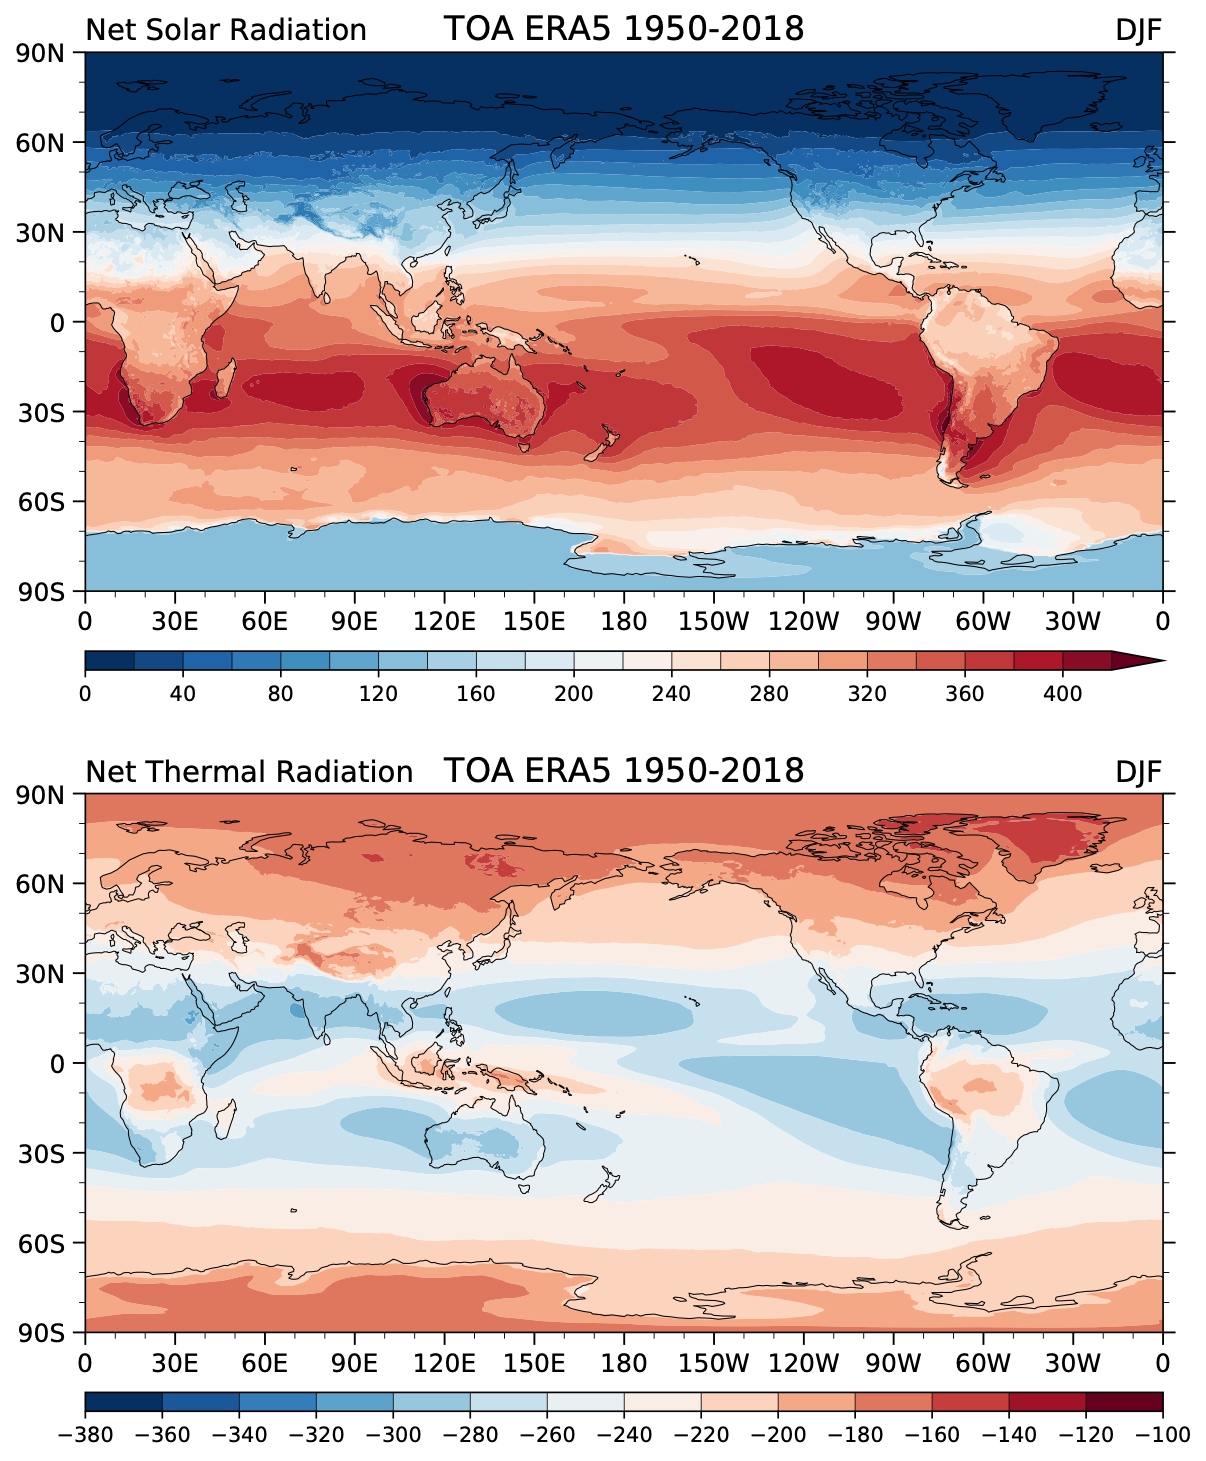
\includegraphics[width = .7 \textwidth]{figs/GD/TOADJF.png}
\caption{} \label{fig:}
\end{figure}

% . {[}fig:750{]}

The climatological distribution of the radiation at the top of the
atmosphere is shown in Fig.(\texttt{fig:750}). The picture represents
the situation for boreal winter (DJF). The arctic night is visible and
it is possible to notice it in the progressively decreasing flux of
solar radiation towards the North Pole, eventually reaching zero. The
Southern Hemispherewill show a similar picture in boreal Summer (JJA).
The flux shows a predominantly latitudinal structure following the
spherical geometry of the planet, but significant asymmetries are
visible in the Equatorial area, where there are large region of reduced
flux caused by the presence of highly reflective clouds. The extensive
snow and ice coverage of Antarctica creates a similar reduction in the
summer hemisphere. The vast regions of high flux are basically
cloud-free zones where the lower layers of the atmosphere or even the
surface are directly visible from space.

The bottom panel of the figure shows the thermal radiation. Starting
from the Equatorial region we can notice in the Maritime Continent a
region of low flux, caused again by the high clouds top that induce a
relatively cold radiative surface towards outer space. The tropical
region is basically a desert area with few clouds and intense direct
radiative flux from the Sun.

It is interesting to consider the difference between precipitation and
evaporation (Fig. \texttt{fig:70aa}). The evaporation is maximum in the
subtropical region and it is minimum in the equatorial region. The net
balance, evaporation minus precipitation, \(E-P\) is positive in the
subtropics, indicating a net loss of water from this region towards the
mid-latitudes and towards the Equator.

\begin{figure}
\centering
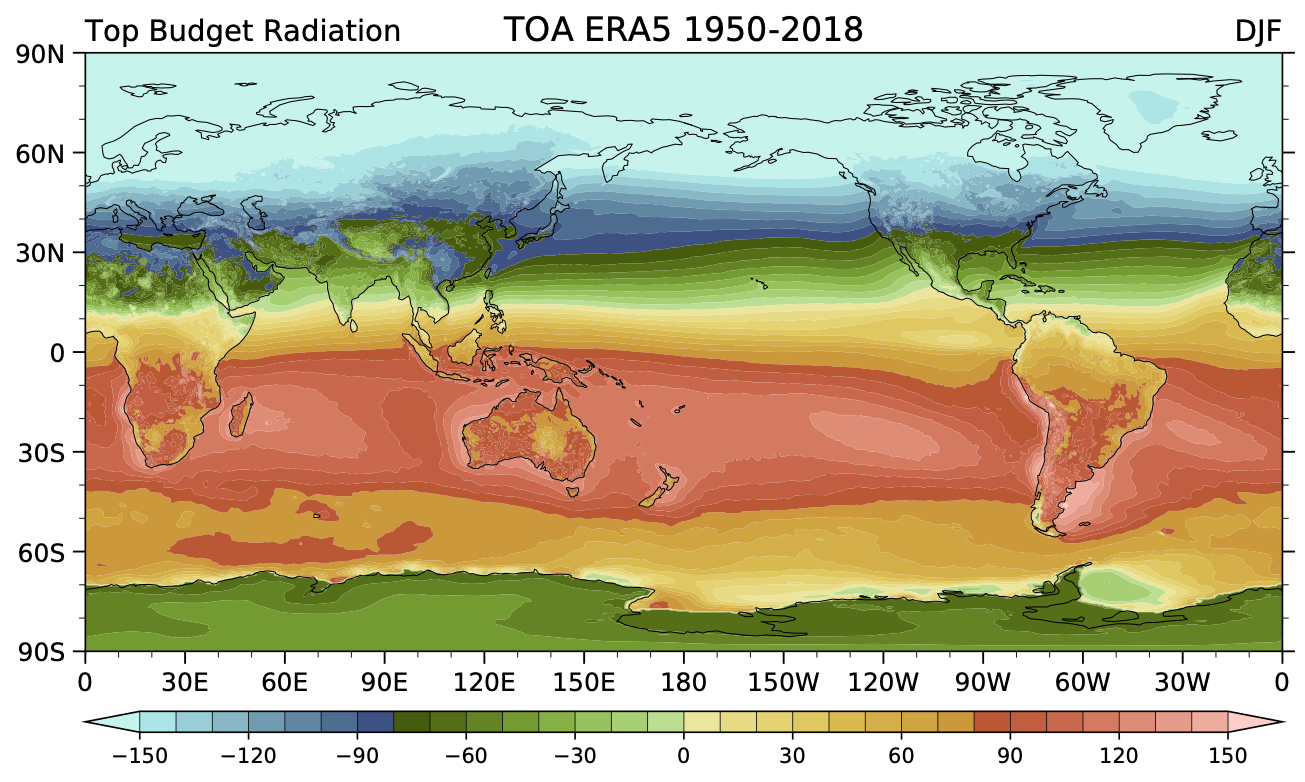
\includegraphics[width = .7 \textwidth]{figs/GD/TOABudgetDJF.png}
\caption{} \label{fig:}
\end{figure}

. {[}fig:751{]}

The net budget is shown in Fig. \texttt{fig:751}. The outgoing flux is
dominated by the Summer hemisphere, but there is a significant radiation
loss also in the Arctic that in this season receives almost no solar
radiation. It is possible to notice that along the southern Tropic there
is instead a large surplus of incoming radiation flux. The situation
points to a gain of radiative energy in the tropical region (for this
season mostly the southern Tropic) and a net loss in the polar region,
in this case the Arctic. Noting the predominant zonal structure of the
distribution in this figures it is probably useful to have a look at the
zonal mean of these quantities for both seasons and the whole year. Such
zonal means are shown in Fig. \texttt{fig:752}. The annual mean solar
radiation is not perfectly symmetrical showing some deviations from the
expected astronomical behaviour, also the thermal radiation is showing
variations that are due to the dynamics.

The net balance is showing a surplus of radiative flux in the
subtropical regional and a deficit in the polar regions. The global
radiation budget can be obtained by integrating over the surface of the
Earth the radiative fluxes. The polar region have smaller area and so
they will contribute less to the integral, but the results is the global
integral of the solar radiation, annual mean, is 242.963 \(W m^{-2}\)
and for the thermal radiation is -242.673 \(W m^{-2}\) for a global
budget of 0.290 \(W m^{-2}\), an almost perfect balance. Over the 70
years of the reanalysis period the error is less than 3/10 of a Watt.

\begin{figure}
\centering
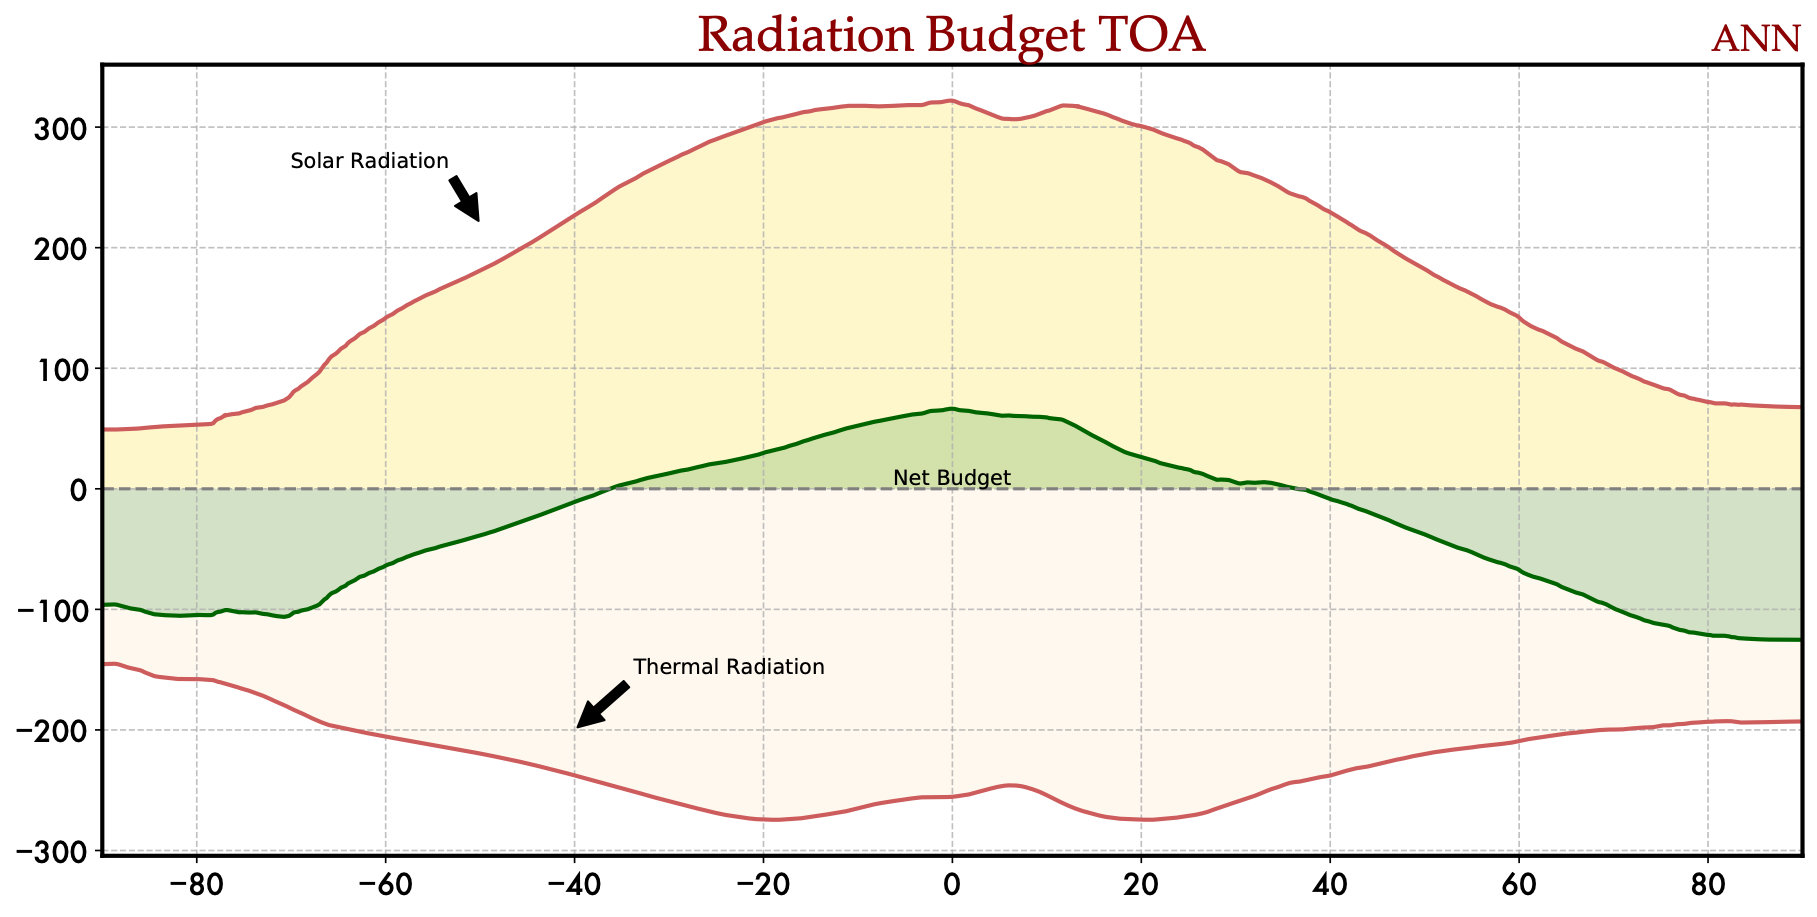
\includegraphics[width = .7 \textwidth]{figs/GD/BudgetTOAANN.png}
\caption{} \label{fig:}
\end{figure}

\subsection{The surface energy
balance}\label{the-surface-energy-balance}

At the surface the energy balance involves more processes. There is also
here a net solar radiation flux, modulated by the albedo of the surface
and of the atmosphere and a net thermal flux, obtained as the balance
between the radiation emitted by the surface and the downward flux
coming from the bulk of the atmosphere. Then there is a sensible heat
flux caused by the turbulent vertical motion that carry away heat
through mechanical agitation and the latent heat flux that represent the
heat necessary for the evaporation of water from the surface. Because of
the extent of the Ocean the latent heat flux is an important element of
the budget.

The annual surface radiation budget is shown in Fig. \texttt{fig:760}.
The long wave flux is the result of combining the upward thermal flux
from the surface and the downward thermal flux from the atmosphere. The
sign convention is such that negative fluxes represent fluxes away from
the surface so that we can see that the deserts and elevated areas (the
Tibetan plateau, the Rocky Mountains) are strong emitters of long wave
radiation, whereas most of the ocean is relatively less active.

For the short wave budget (lower panel) the sign is everywhere positive,
indicating that everywhere the flux is in the surface, but the polar
regions are receiving on the annual mean a small amount of short wave
radiation, once you take into account the dark winters. The subtropical
regions are those that receive the strongest insulation even with
respect to the Equator. it is clear that clouds here play an important
role.

\begin{figure}
\centering
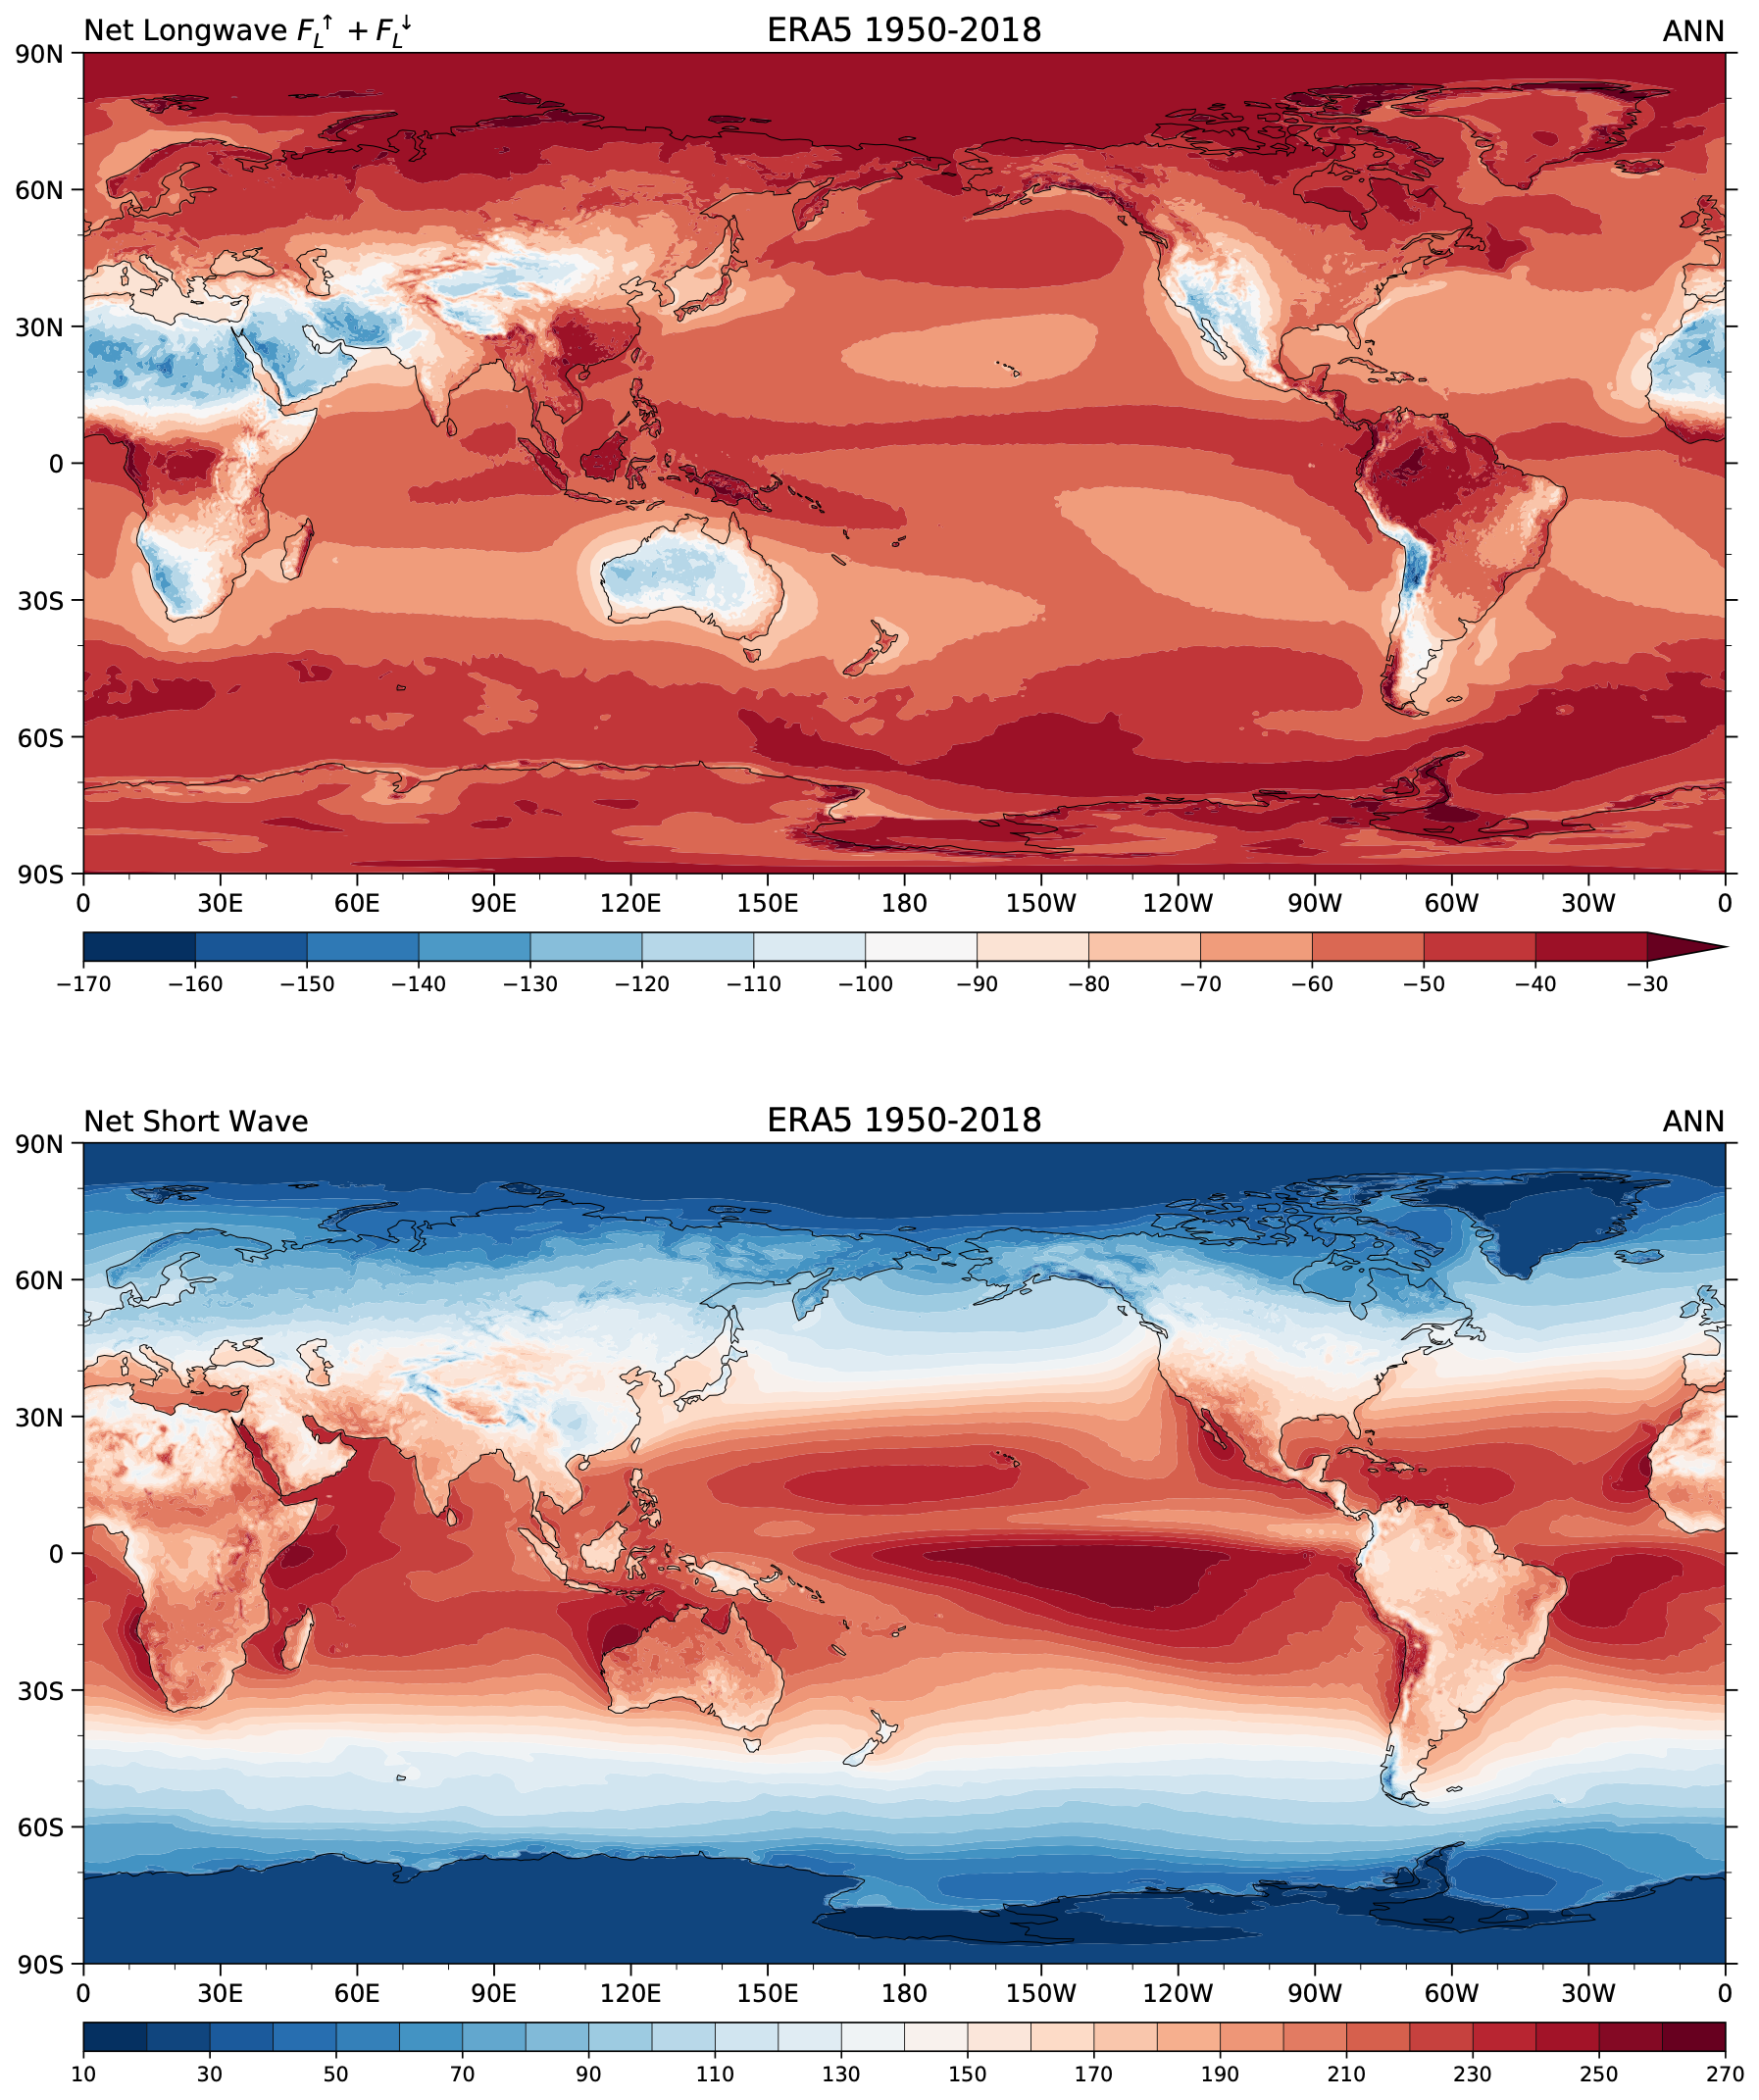
\includegraphics[width = .7 \textwidth]{figs/GD/SrfRadANN.png}
\caption{} \label{fig:}
\end{figure}

The heat fluxes are instead shown in Fig. \texttt{fig:761}. The sensible
heat flux (upper panel) represents transfer of heat by conduction and
turbulent fluxes in the vertical. The ocean show a positive sensible
heat flux, indicating that they tend to be warmed by these fluxes,
whereas the land exhibits a marked heat loss. The high latitude, high
elevation areas in Greenland and Antarctica have a lso a positive heat
flux. The boundary currents regions off the east coast of North America
e Japan are also regions of heat loss.

The latent heat flux (lower panel) shows very interestingly that the
major latent heat loss in the subtropical oceans and in the boundary
current areas, whereas land contributes less to the latent hear release.
The polar regions have very small fluxes from latent heat loss.

\begin{figure}
\centering
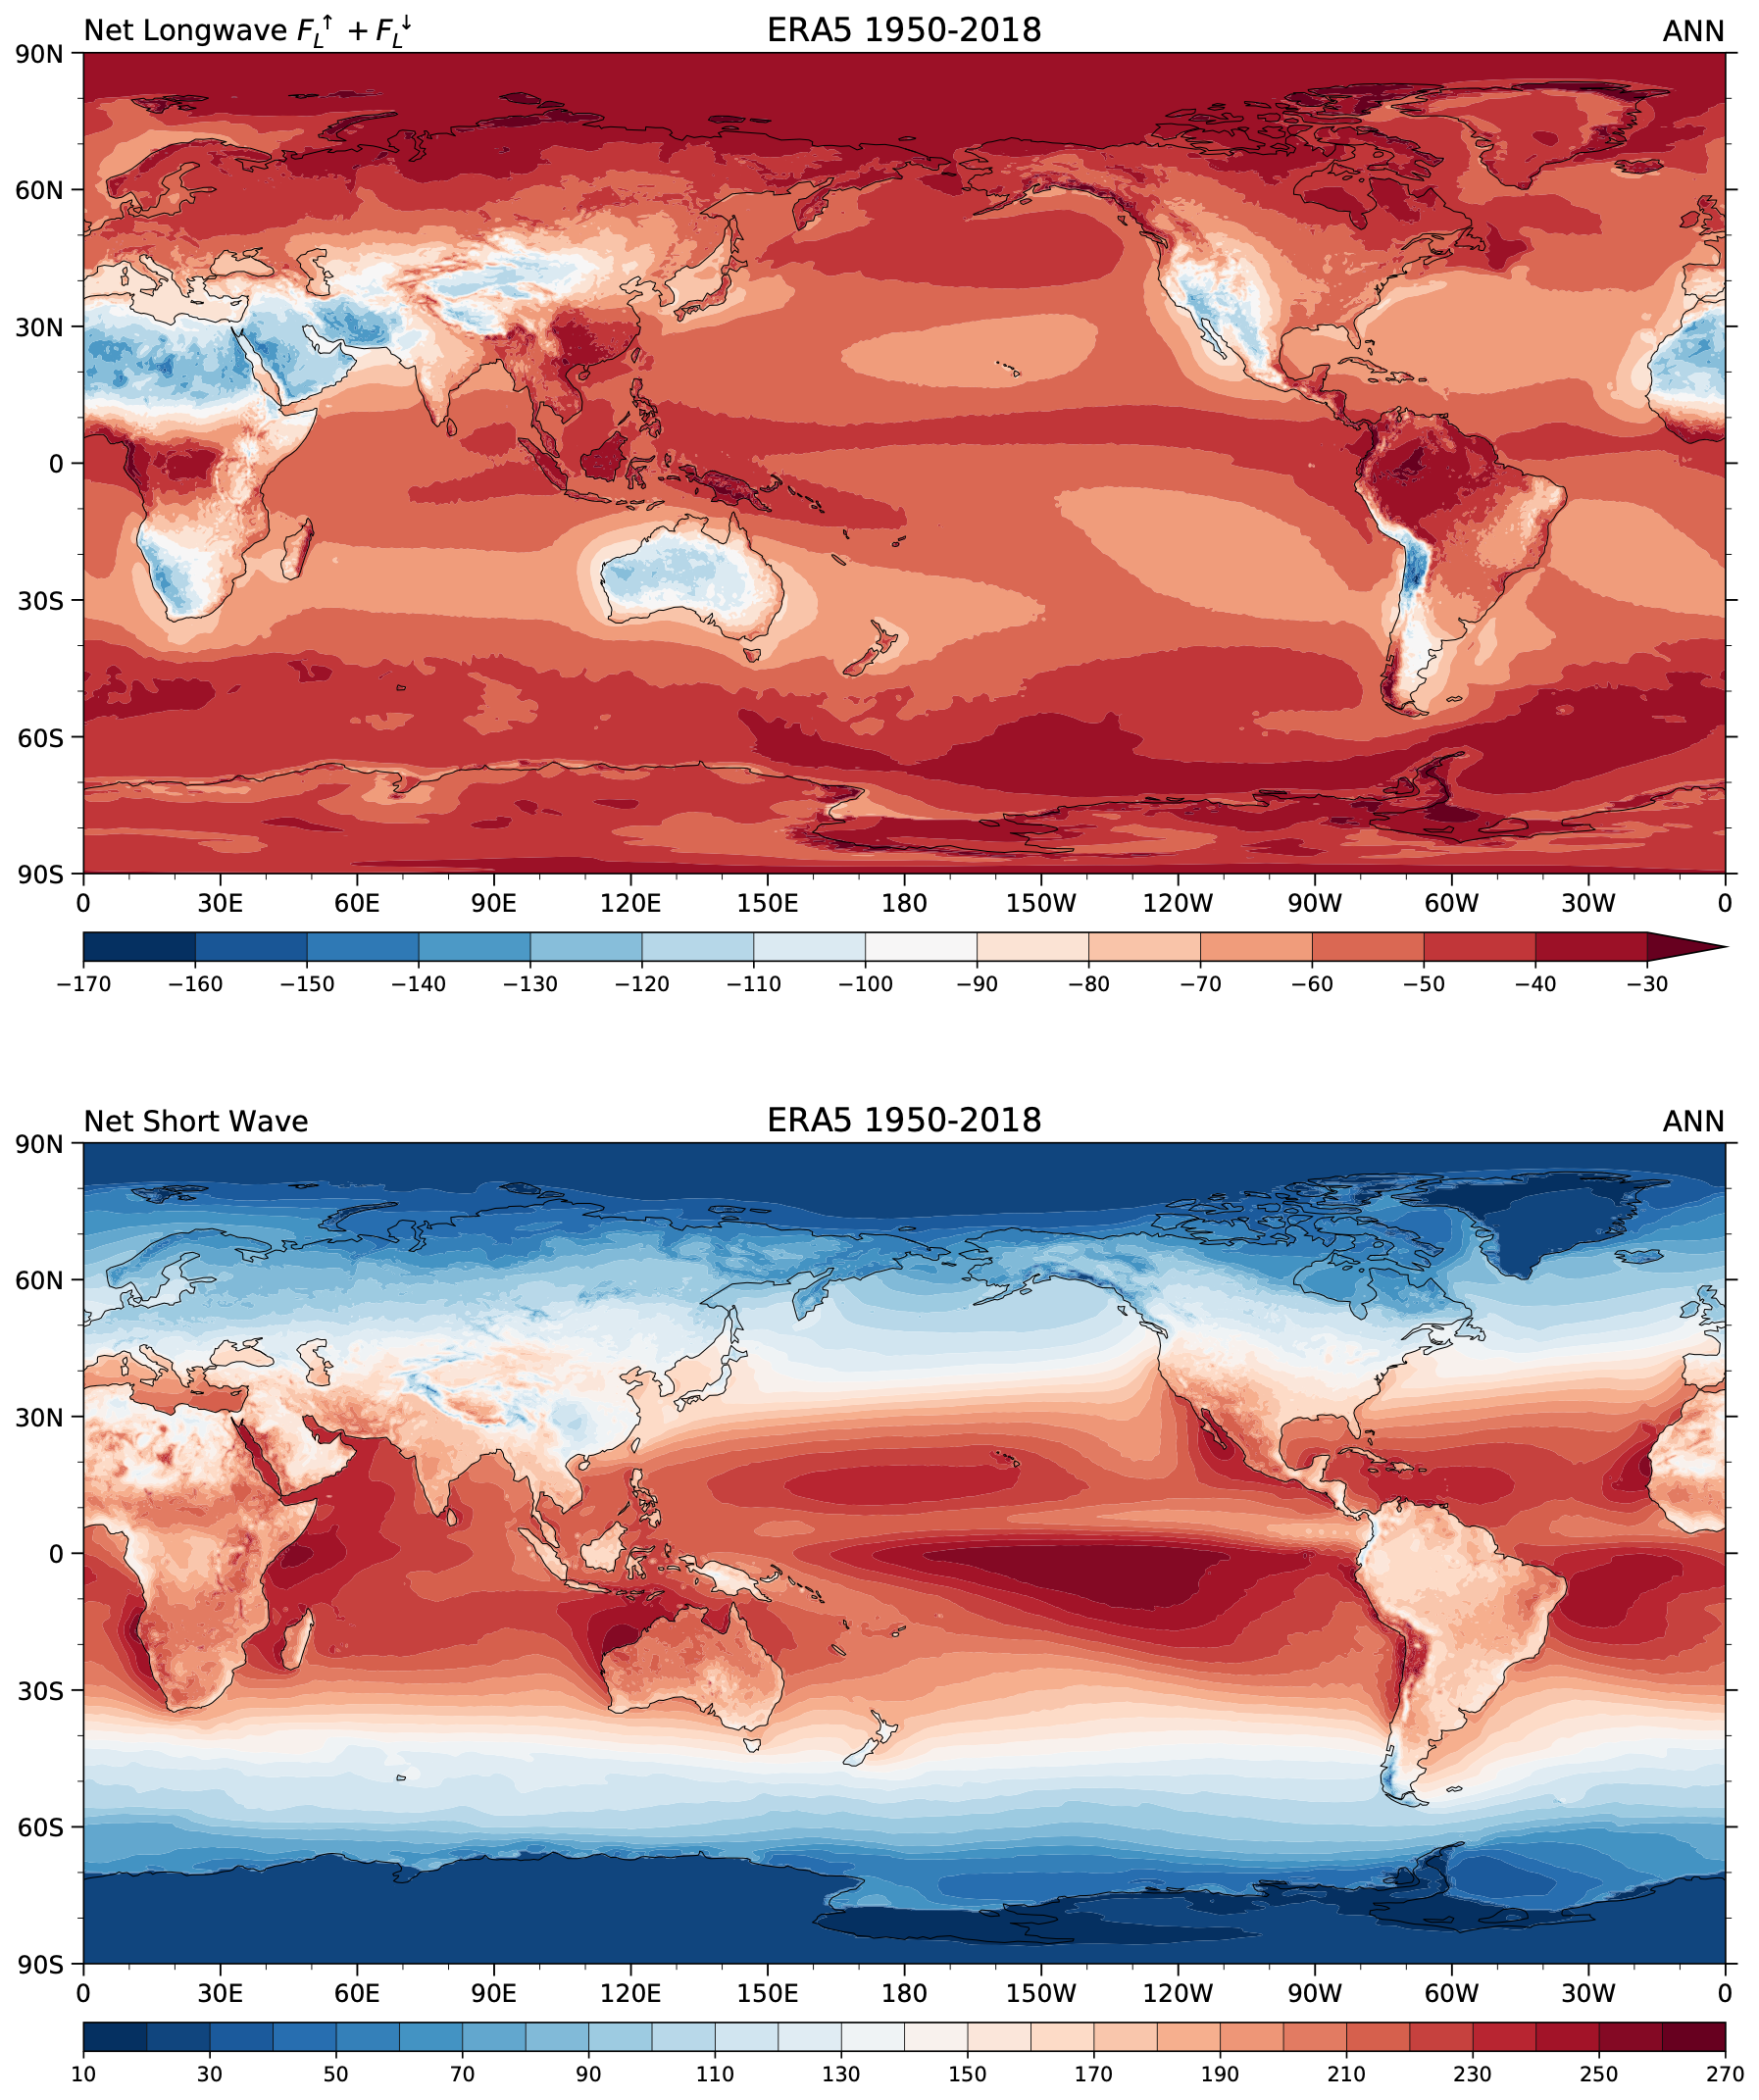
\includegraphics[width = .7 \textwidth]{figs/GD/SrfRadANN.png}
\caption{} \label{fig:}
\end{figure}

Putting together all the terms of the budget we obtain Fig.
\texttt{fig:763}. Here we are showing the complete budget

\[F_L^\uparrow + F_L^\downarrow + F_{SH} +F_{LH} \approx 0\]

The first comment is that in general terms the surface acquires heat at
low/equatorial latitudes and loses heat at high latitudes. The North
Atlantic especially is a site of large heat loss together with the
Antarctic region. There is a strong heat gain in the equatorial area,
especially in the Pacific, with a peak in the East Pacific.

\begin{figure}
\centering
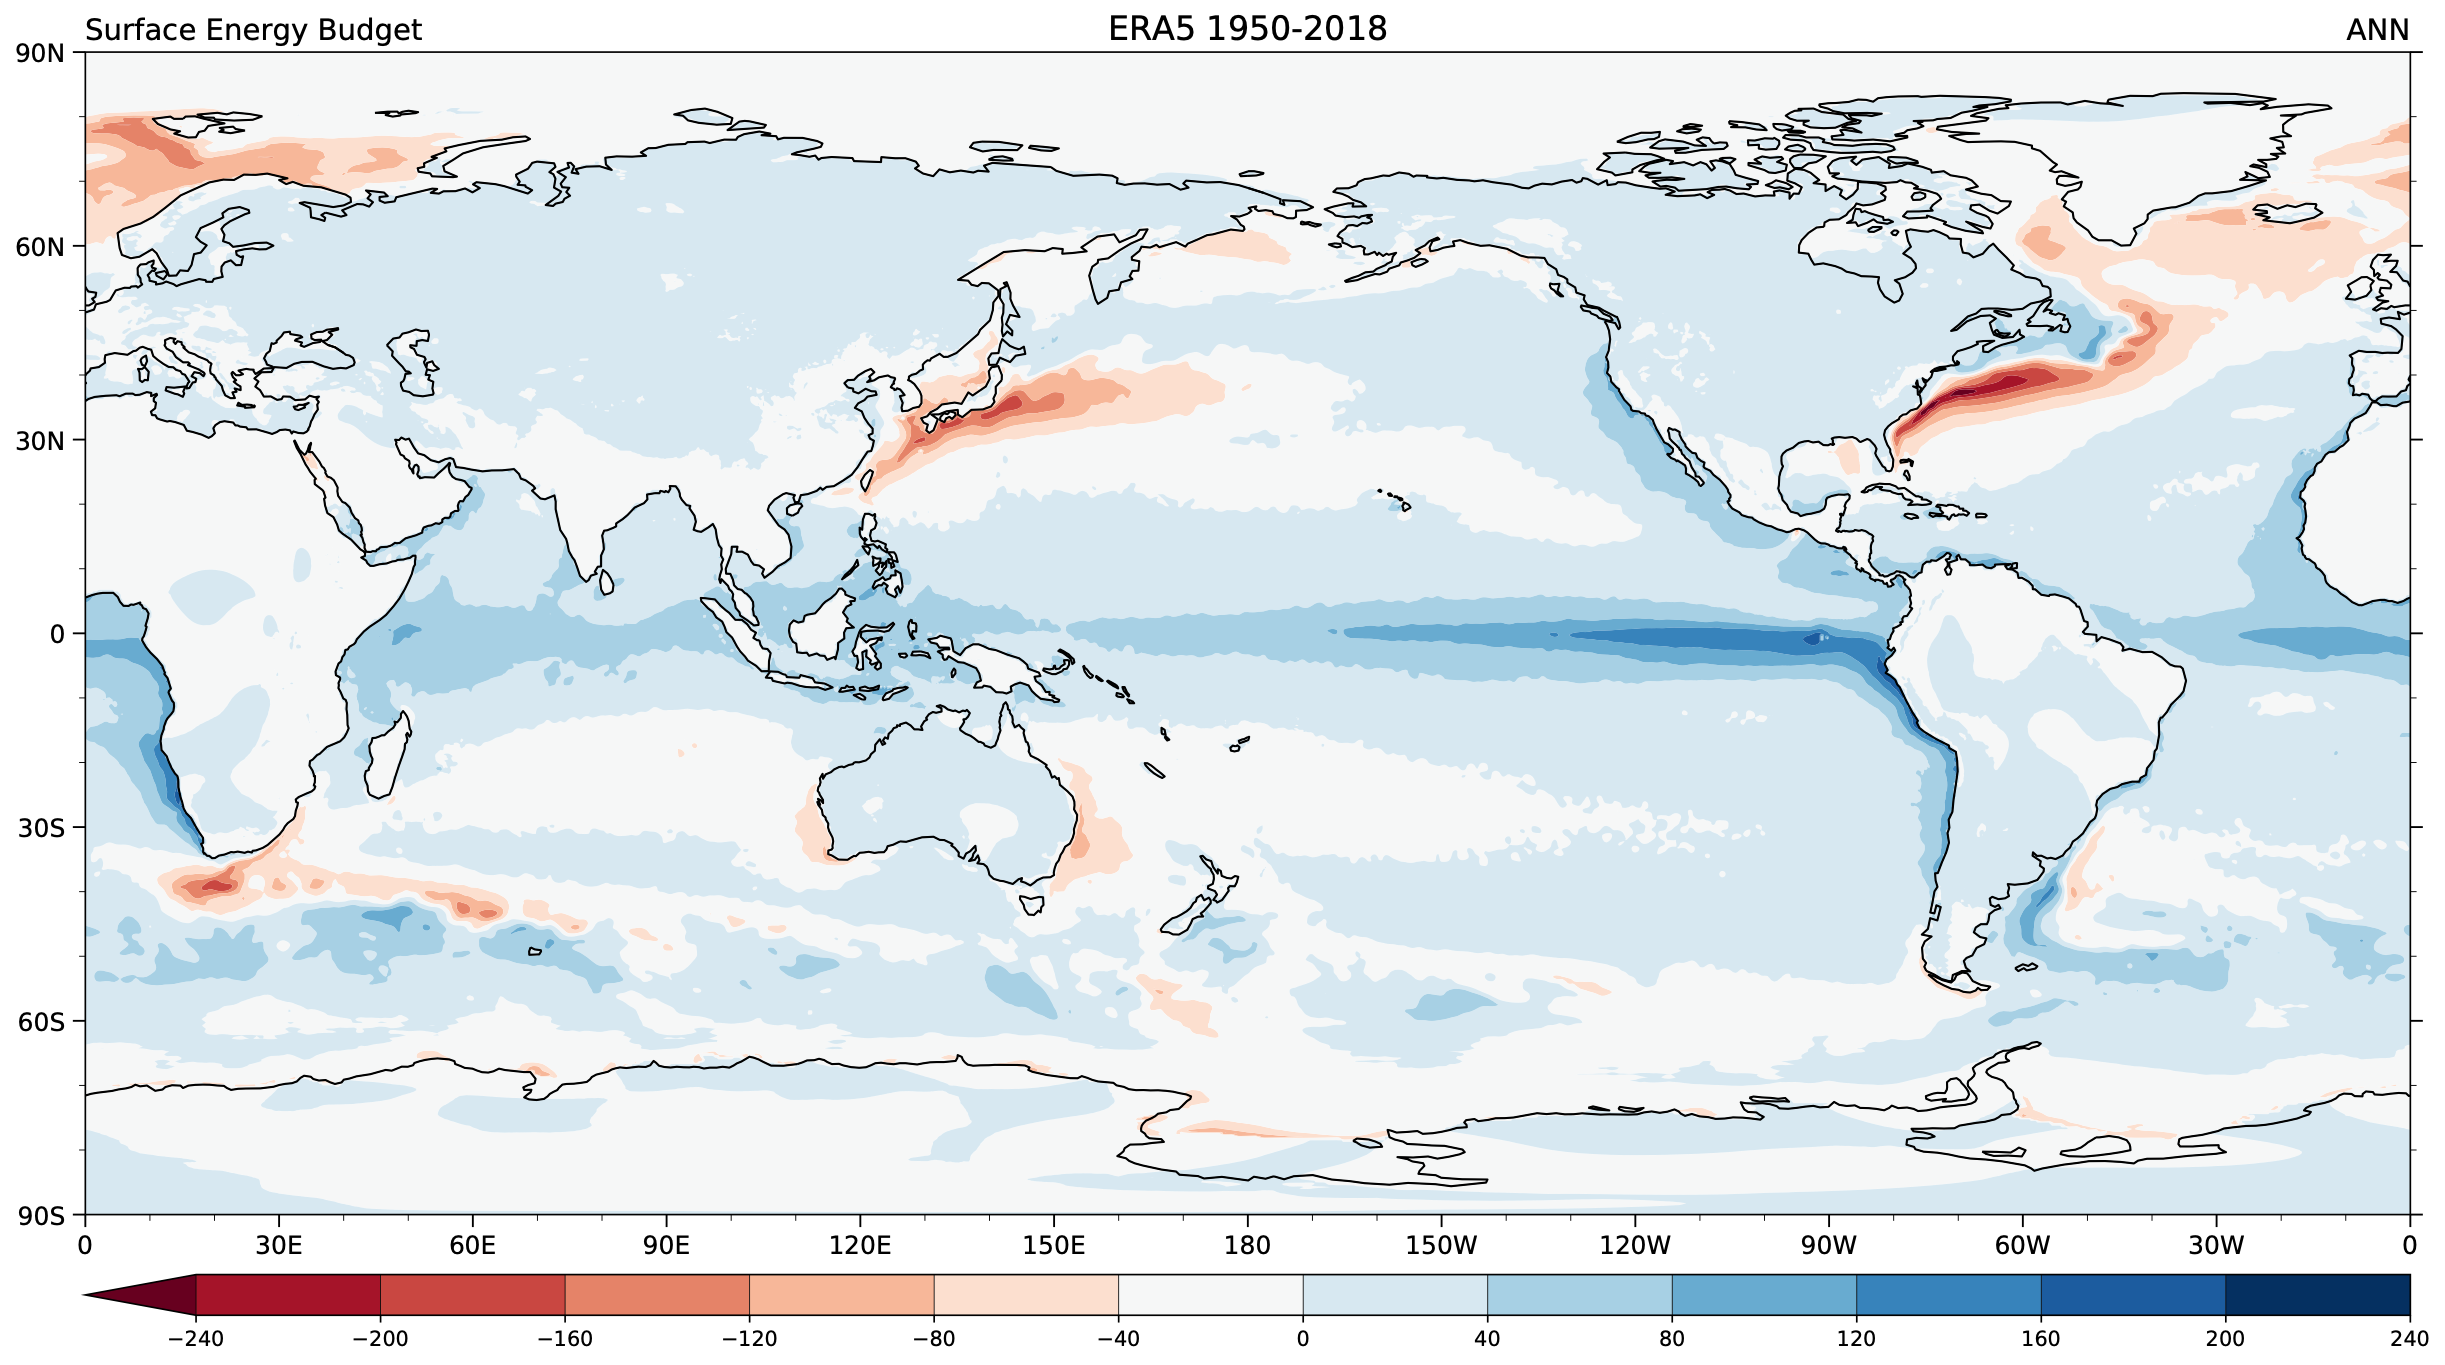
\includegraphics[width = .7 \textwidth]{figs/GD/SrfBudgetANN.png}
\caption{} \label{fig:}
\end{figure}

Summarising the budget in the zonal mean, we can see from Fig.
\texttt{fig:762}. The excess radiation in the equator is clearly
visible, together with the massive loss for latent heat peaking off
equator. The latent heat flux becomes negligible in the polar region and
in the sout polar region there is almost local compensation between the
radiation and sensible heat. The north pole is different and residual
latent heat is visible, probably linked to the larger amount of ice-free
ocean that especially in the Summer is present in the Arctic. The net
budget indicates a clear zonal imbalance with the equatorial areas
gaining heat and the midlatitudes losing heat. The analysis does not
distinguish between land and ocean, but because the oceans are two third
of the Earth surface it is clear that the dominant effect here is
transfer of heat to and from the ocean. The land equilibrates on a much
faster scale and therefore eliminate quickly imbalances by adjusting the
temperature.

\begin{figure}
\centering
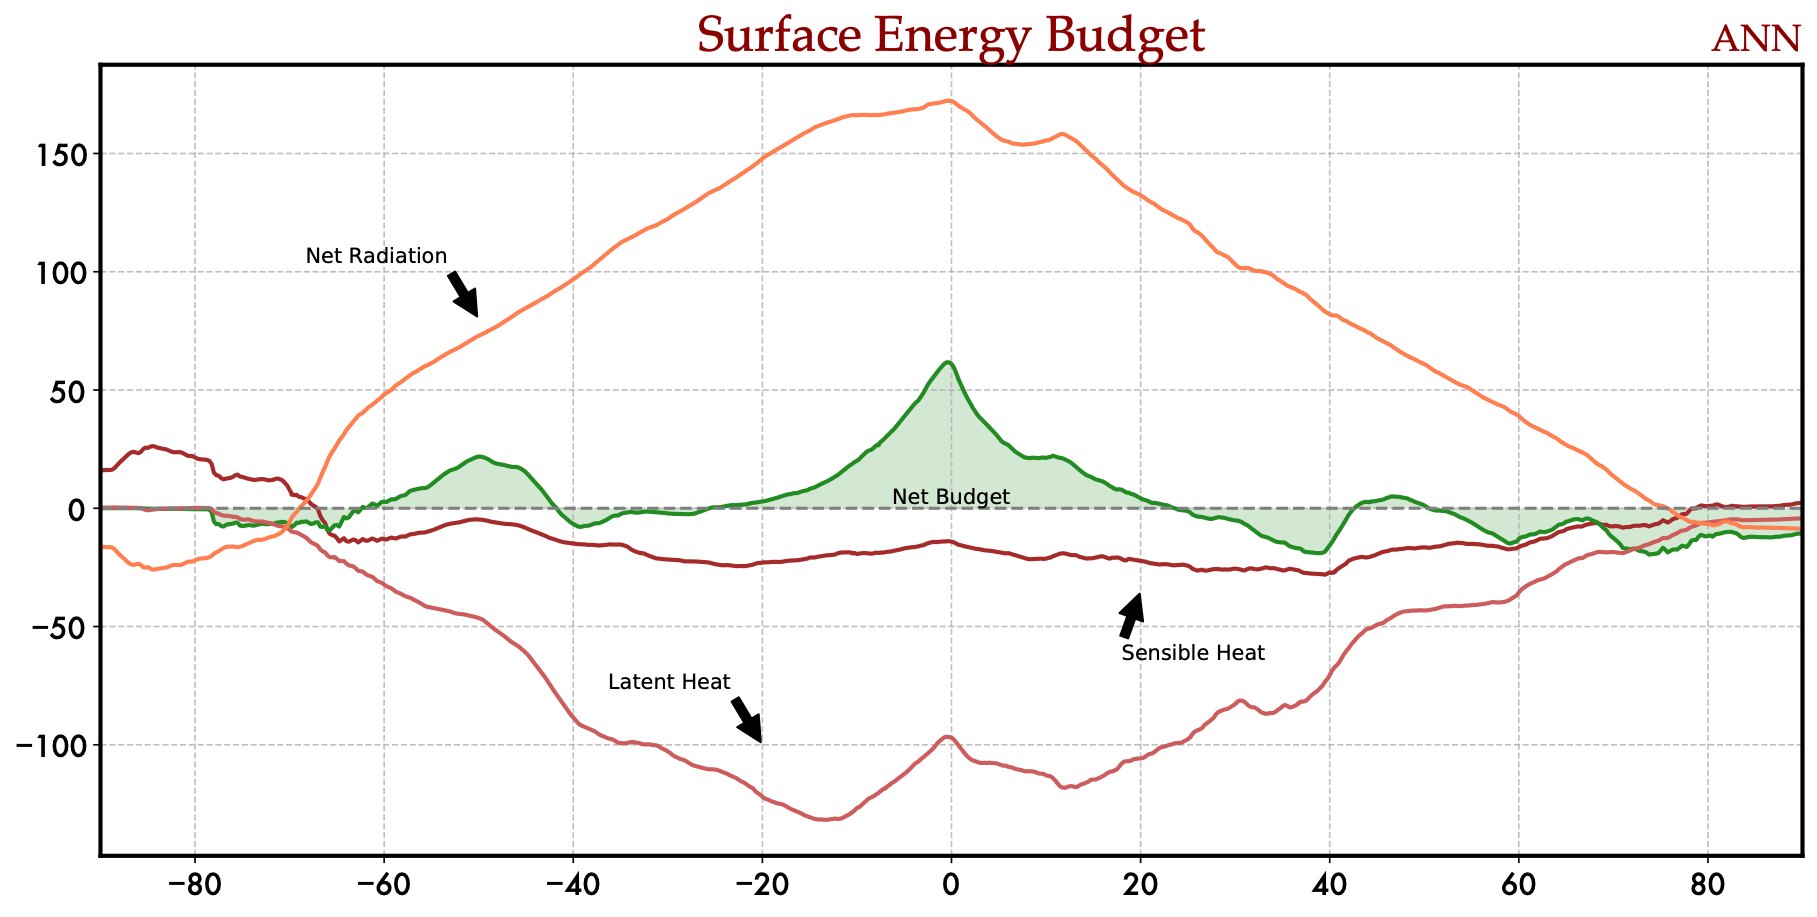
\includegraphics[width = .7 \textwidth]{figs/GD/SrfBudProfileANN.png}
\caption{} \label{fig:}
\end{figure}

Global integration of the fluxes over the Earth yield the following
global numbers: total sensible heat flux -16.838 , latent heat flux
-82.030 , total short wave 164.007, total long wave -58.244 for a global
balance of 6.895 \(W m^{-2}\).

\subsection{Precipitation}\label{precipitation}

The zonally averaged precipitation is shown in Fig. \texttt{fig:70a}. In
general, the precipitation has a maximum in the equatorial zone and
secondary maxima in the mid-latitudes. The maximum at the Equator moves
with the seasonal cycle of the Sun into the summer hemisphere, showing
however an asymmetry, since in Summer it is located around 5N, whereas
in Winter is at 15S. The mid-latitude precipitation is more intense in
winter, but it does not show much of a seasonal cycle.

The compilation of climatological precipitation is a difficult problem,
reflecting the high spatial variability of the precipitation. We show in
Fig. \texttt{fig:61p} shows the climatological precipitation as compiled
by ERA5 reanalyses, butother products are available. For instance, the
GPCP project\footnote{GPCP Precipitation data provided by the
  NOAA/OAR/ESRL PSD, Boulder, Colorado, USA, from their Web site at
  \url{https://www.esrl.noaa.gov/psd/} Adler2003 and atmos9040138 is
providing an independent analysis of precipitation including satellite
and in situ data, on a somewhat coarser resolution grid and only after
1979. Recently a climatology at a higher resolution (0.1 deg) has also
been compiled for the period 1979-2017 BeckMSWEP2019.}

The general structure of the horizontal distribution (Fig.
\texttt{fig:70}) shows narrow belts of intense precipitation in the
equatorial zone. This precipitation is linked to the converging motion
that are visible in the meridional circulation (Fig. \texttt{fig:54}),
the rising air creates conditions that are favourable to the generation
of deep convection. These tropical convergence zones are also known as
the Intertropical Convergence Zone (ITCZ), it is interesting to note
that in the West Pacific a similar line of intense precipitation is
slanting toward the South-East creating a structure known as the South
Pacific Convergence Zone (SPCZ).

\begin{figure}
\centering
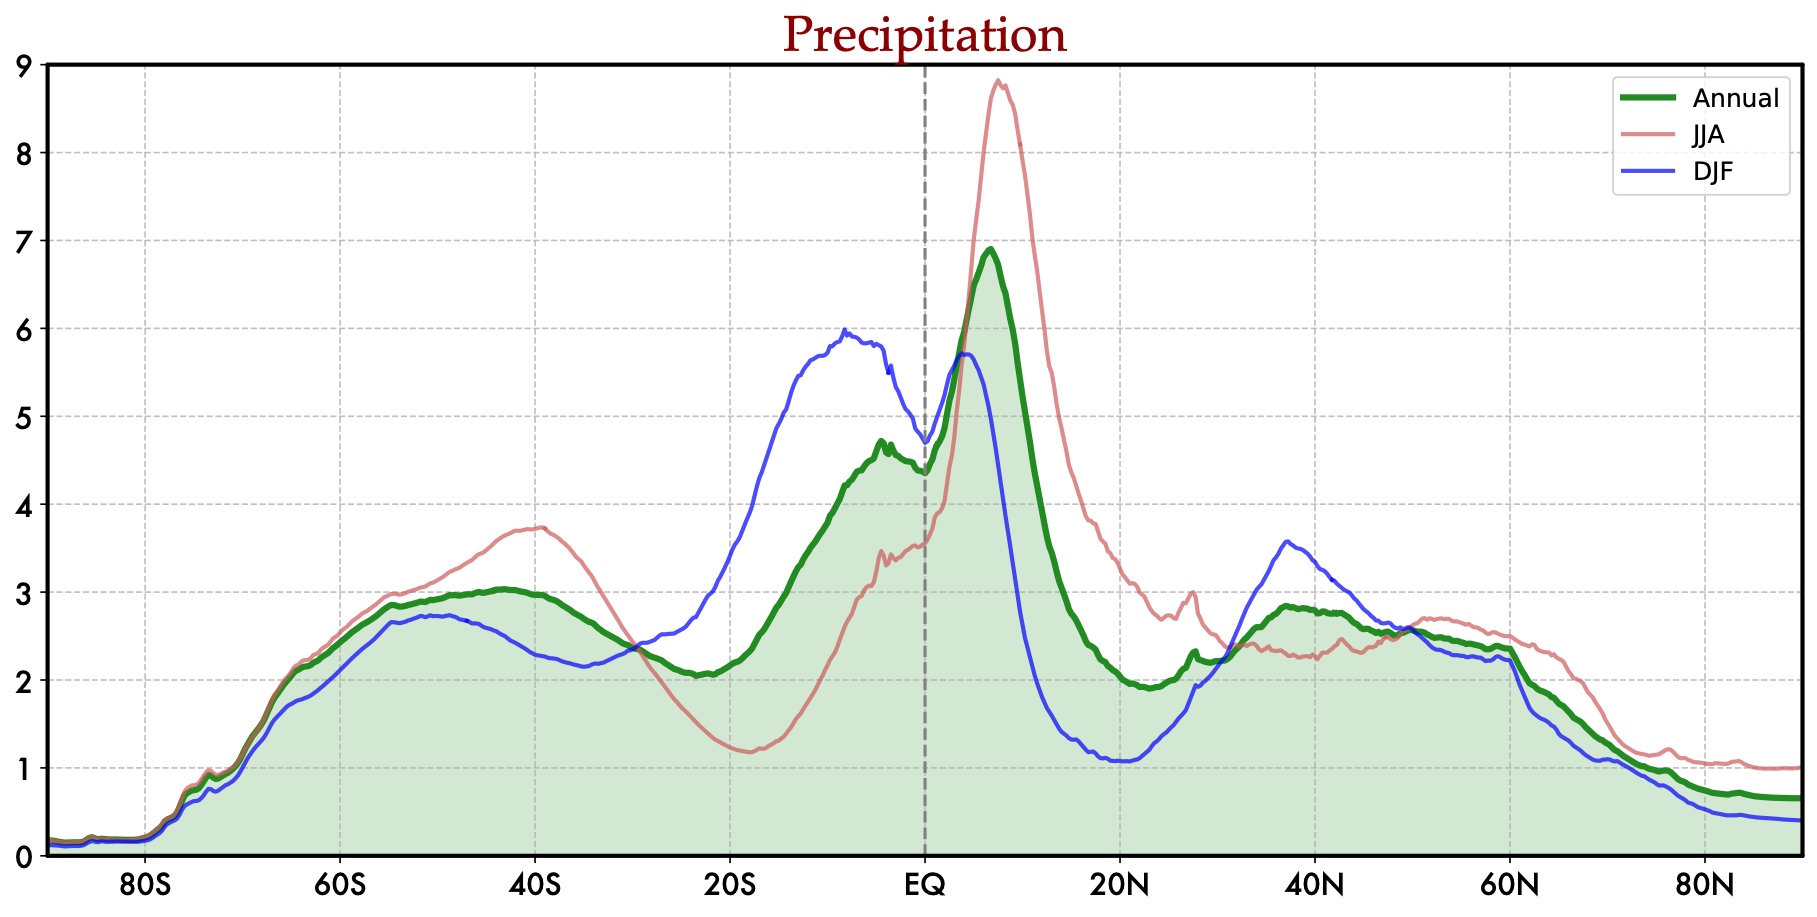
\includegraphics[width = .7 \textwidth]{figs/GD/PrecALLJJA.png}
\caption{} \label{fig:}
\end{figure}

The precipitation in the mid-latitude is aligned along the the preferred
path of developing storms, the storm-tracks. This precipitation is due
to the raising of warm, moist air due to the baroclinic instabilities in
the westerly current of the midlatitudes. Precipitation linked to the
baroclinic storm tracks in Winter can be seen from the East coast of
North America elongating into Europe and the Mediterranean and from the
Asian Far East into the Pacific Ocean.

The Summer monsoonal precipitations of the South Asian Monsoon over
India and Indochina, of the West Africa Monsoon and of the weaker North
American Monsoon are clearly visible. In general, major convective
centers are present over South America and over the Maritime Continent.

\begin{figure}
\centering
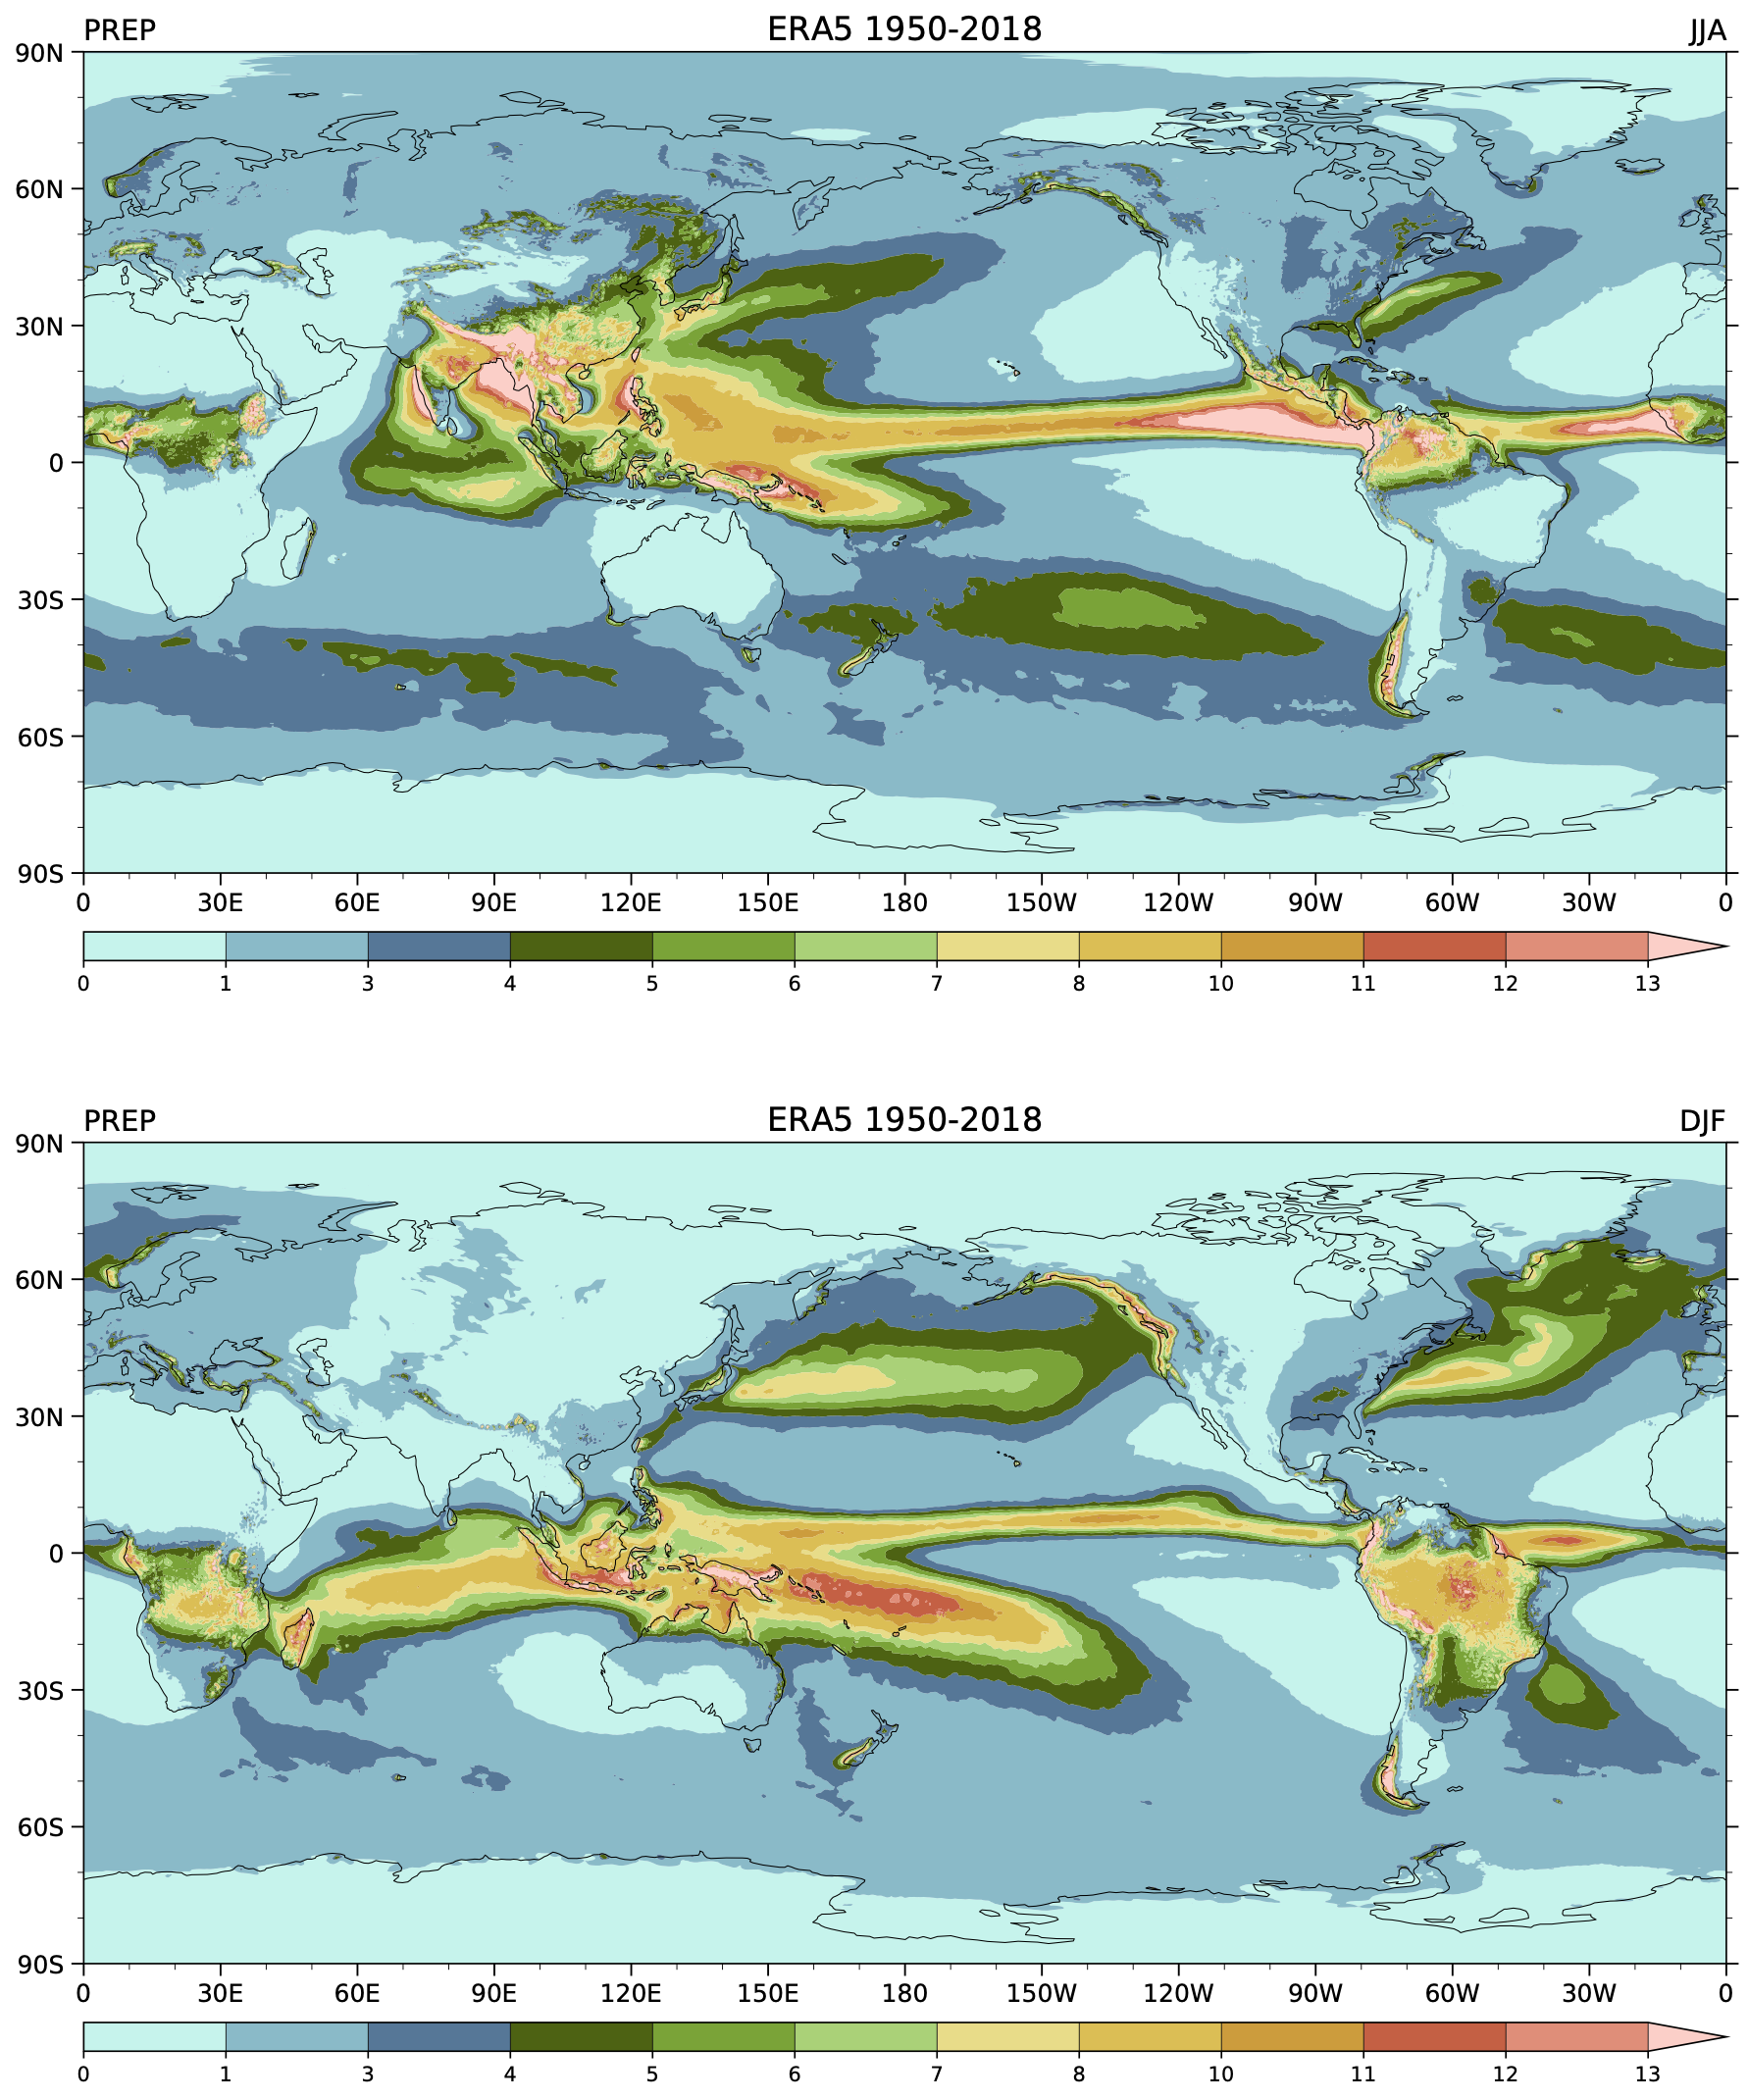
\includegraphics[width = .7 \textwidth]{figs/GD/TPREP.png}
\caption{} \label{fig:}
\end{figure}

The water balance (\emph{hydrological balance}) at the surface will
require that we get estimate of all the components of the balance
equation for water at the surface. Precipitation can be seen as a
downward water flux and the upward water flux is represented by phase
transformation of liquid water in vapor, through a process called
evaporation. Evaporation depends on many factors, including the surface
wind, the water content of the soil, the presence of vegetation. The
elements of the balance therefore will be different over land or over
the oceans. Over land we will need to take into account also of the
liquid water at the surface that goes into river and lakes and
eventually find its way into the sea, the run-off. We need to consider
also the filtration of water into the deeper layer of the soil to go
into the underground reservoirs. Over the oceans the E-P difference is
simpler and it crucially control one of the basic property of sea-water,
\emph{salinity}.

Furthermore, water vapor contain energy that is released when it
condenses as rain, but this process rarely happens in the same place
where evaporation and therefore water vapor found its origin, so water
is powerful energy vector capable of transporting energy over large
distances. A global view of the relation between evaporation and rain
can be obtained from Fig. \texttt{fig:70aa}. The net balance is
providing us with a clear view of what happens. The atmosphere gain
water vapour in the tropical zone and it looses water as rain in the
ITCZ and in the mid-latitude zones. Different processes are responsible
for the condensation processes, the equatorial zone are dominate by deep
convection, whereas the midlatitudes a precipitation come mostly from
synoptic baroclinic activity.

\begin{figure}
\centering
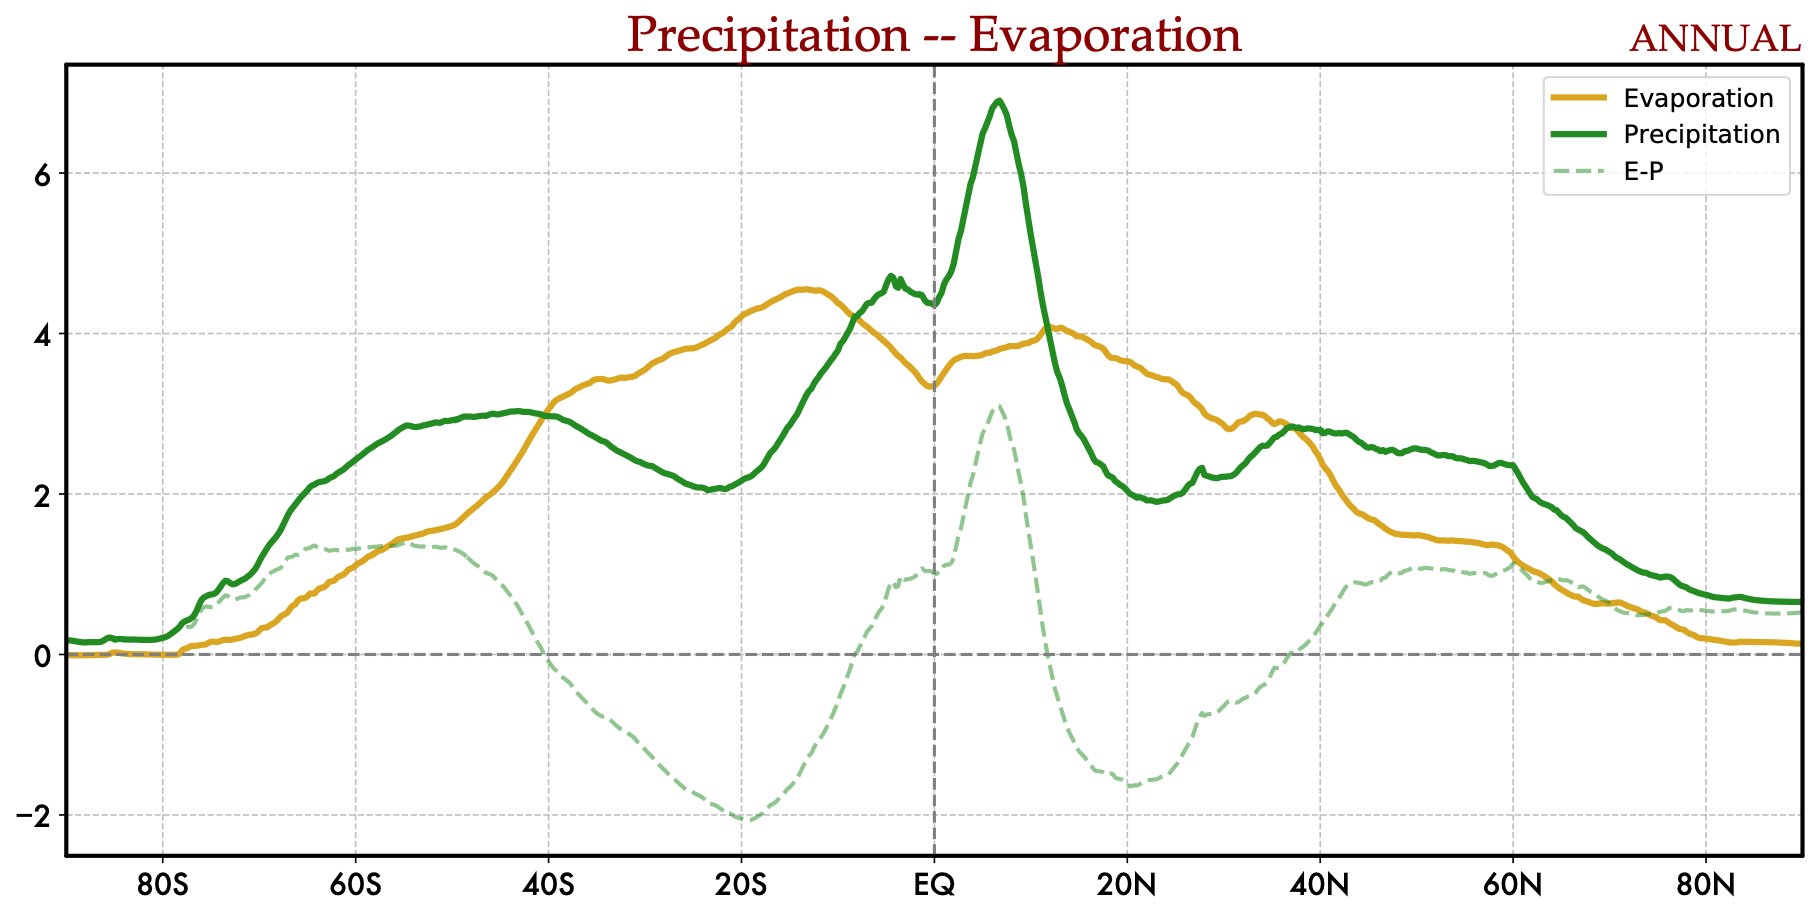
\includegraphics[width = .7 \textwidth]{figs/GD/PrecEvapALLJJA.png}
\caption{} \label{fig:}
\end{figure}

\subsection{Clouds}\label{clouds}

Clouds influence the climate in many ways, the major mechanisms are the
formation of condensation and the removal of water vapor from the
atmosphere through rain, that releases vast amount of energy in the
process, and the scattering, absorption and remission of radiation that
in fact shape very much the energy budget of the planet. Clouds are also
important because they are major player in microphysics of atmospheric
components, aerosols and in the chemistry of the atmosphere. It is
therefore important that we look also at the distribution of clouds.
Compiled data sets of clouds can be obtained by several observational
platforms, but we will use here the product from ERA5 that allows us
also to investigate the vertical structure of clouds.

Fig. \texttt{fig:770} show the cloud distribution in Winter (DJF) in
terms of the fraction of sky occupied by clouds. Clouds can occur at any
level in the atmosphere and the processes that are dominant in each
layer can be different. We are showing here the clouds aggregated in
three layers: (i) high clouds, meaning the clouds that are present above
the pressure level of 45\% of the surface pressure, about 6km, (ii)
middle clouds, aggregating the layers between 45\% and 85\% of the
surface pressure, basically between 6 and 2 km height and then the lower
clouds, namely the layer between the surface and the pressure level of
80\% of the surface pressure, about 2 km. The lower cloud include then
clouds that forms at the border of the planetary boundary layer.

We can see from the picture that the high clouds are dominant in
equatorial and subtropical zone over equatorial Africa and South America
and the Maritime Continent. There are very few high level clouds along
the tropics that confirm once again their nature of a desert zone. There
is a remarkable exception in the equatorial East Pacific where a large
cloud-free zone contrast with the almost total presence of clouds in the
West Pacific. Middle clouds are to be found in the mid-latitudes and
especially over mountains and the East Coast of continents. Lower cloud
are typical of the polar regions in both hemispheres, with the notable
exception of the East coasts of continents that show a large amount of
low clouds.

The Summer situation shows the Northern shift of the ITCZ and high
clouds are now dominant over the Indian subcontinent and Indochina,
connected to the Summer Monsoon, and over Central America. The lower
clouds now appear over the ocean in the Northern Hemisphereand they are
even stronger along the Pacific South American coast and along the east
coast of Africa.

\begin{figure}
\centering
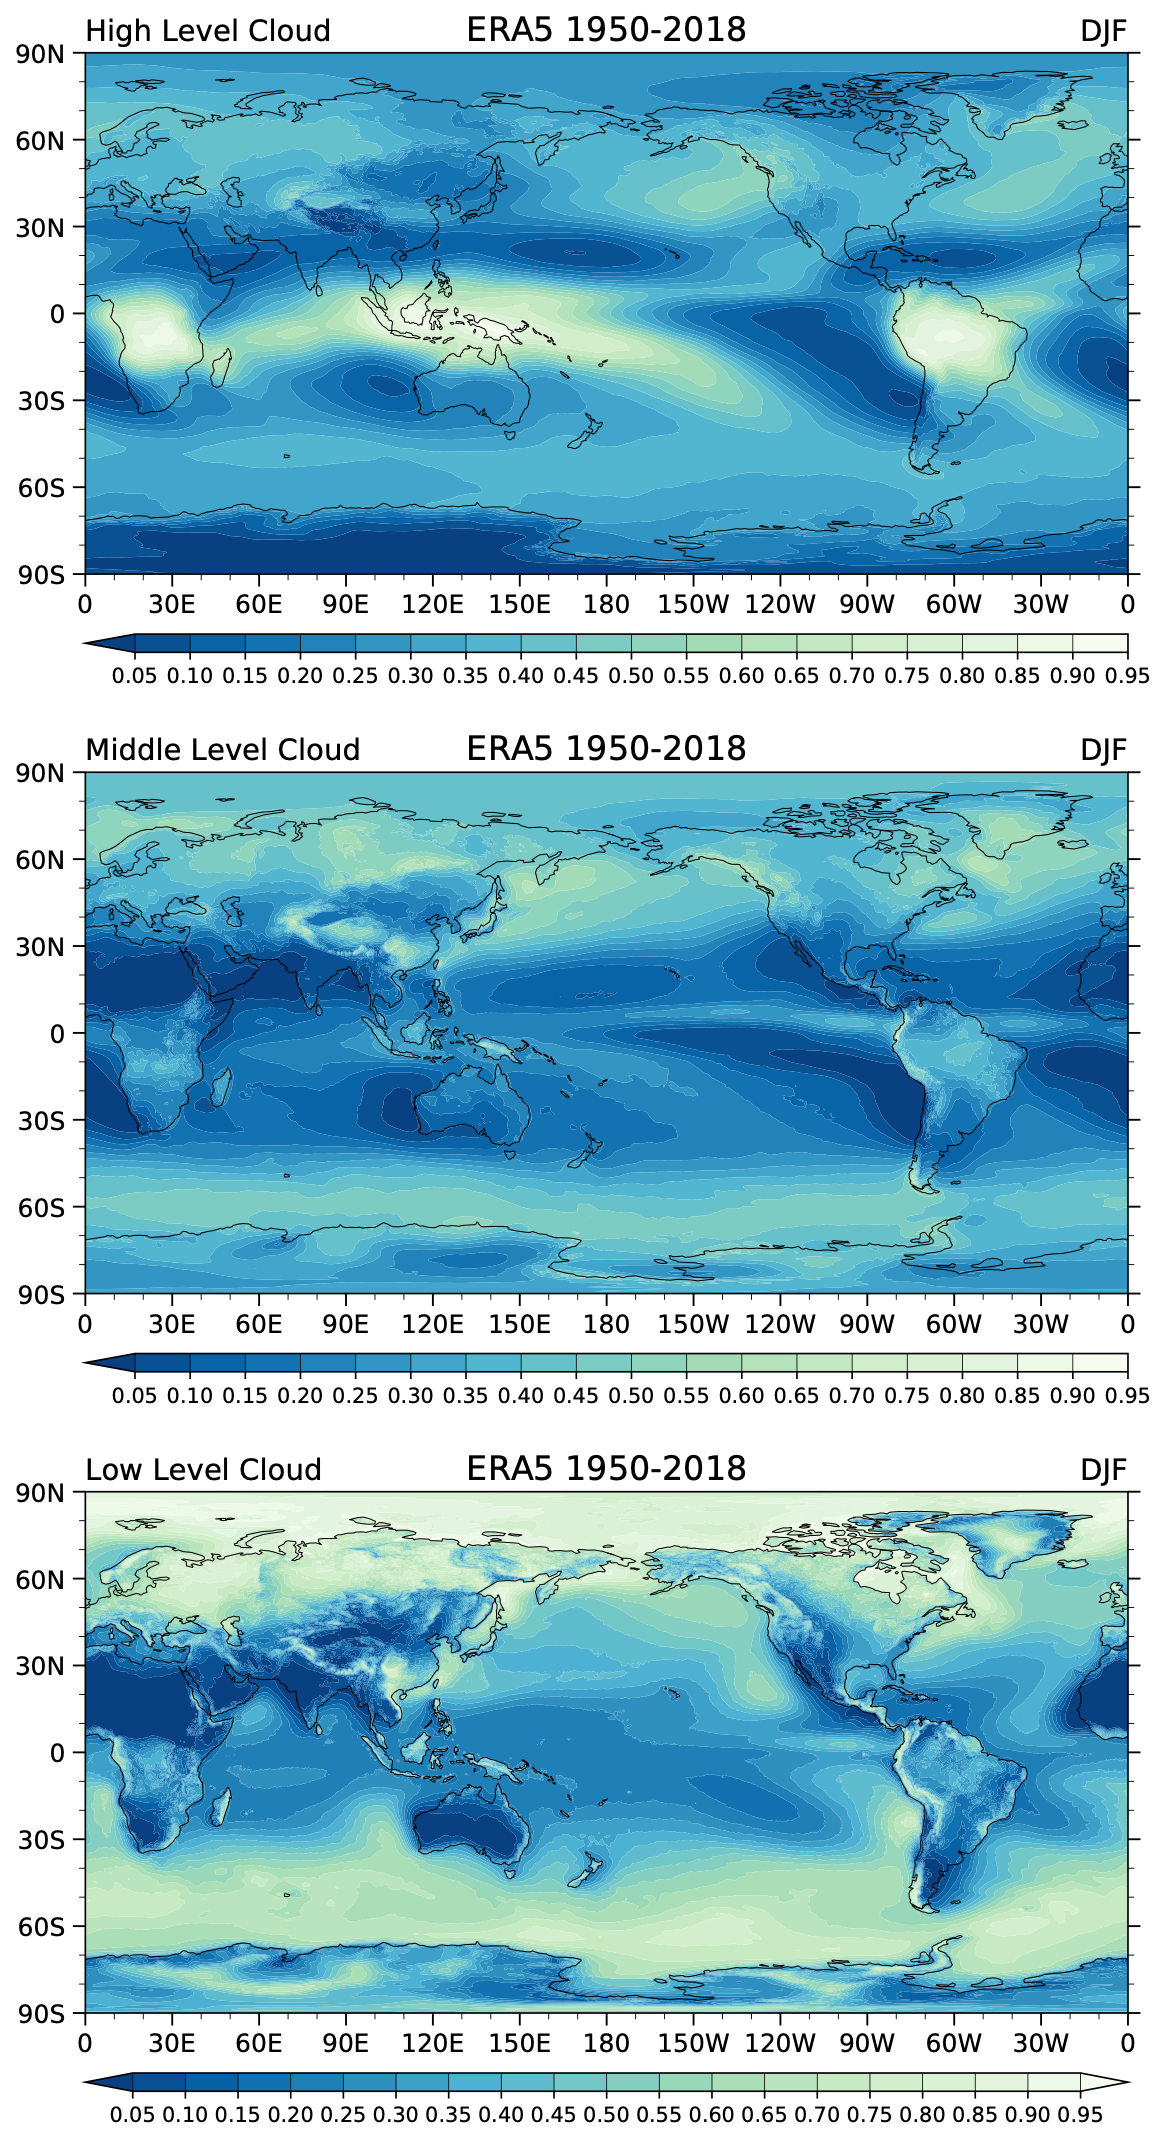
\includegraphics[width = .7 \textwidth]{figs/GD/CloudsLevelDJF.png}
\caption{} \label{fig:}
\end{figure}

\begin{figure}
\centering
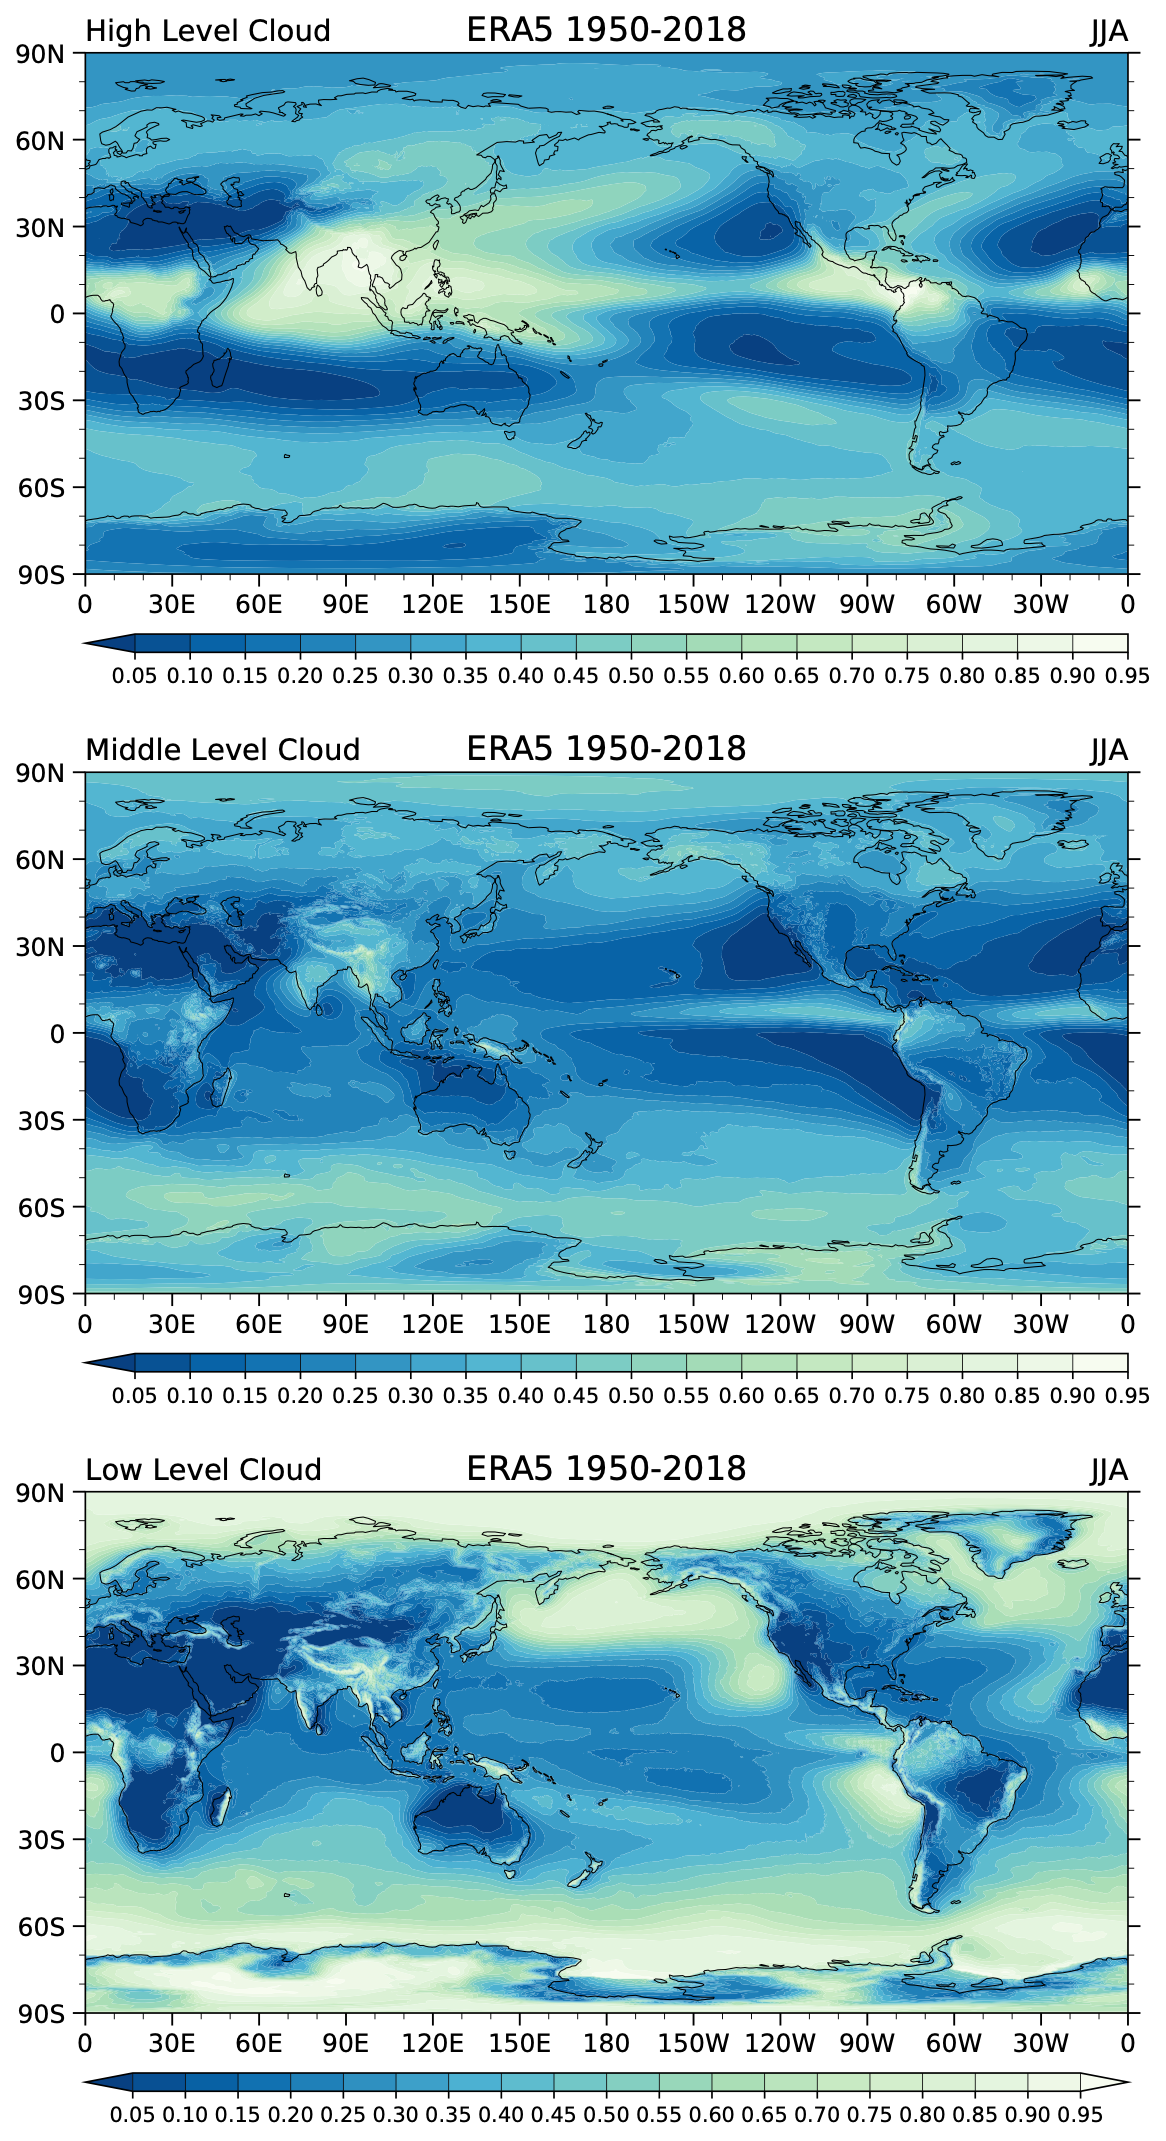
\includegraphics[width = .7 \textwidth]{figs/GD/CloudsLevelJJA.png}
\caption{} \label{fig:}
\end{figure}

Putting everything together we can look at the total cloud cover that is
essentially the aggregated quantity of clouds at various levels. This is
the quantity that is intuitively linked to the observation of a "cloudy
sky". In general clouds are present over a vast surface of the globe.
Some areas show a persistent absence of cloudiness over the entire year,
such as the Sahara desert, part of the Arabian peninsula, Australia and
South Africa. Other areas instead show a strong seasonal cycle, with
different could cover in different seasons. It is interesting to note
that the seasonal cycle takes different chatacteristics in different
areas. In the mid-latitudes cloud cover is larger in the local
hemispheric winter than in the summer. See, for instance the
Mediterranean region and part of the North America West coast. Over
India instead it is the opposite and there are clouds in the Summer
rather than in the Winter (Fig. \texttt{fig:772} and \texttt{fig:773}).

\begin{figure}
\centering
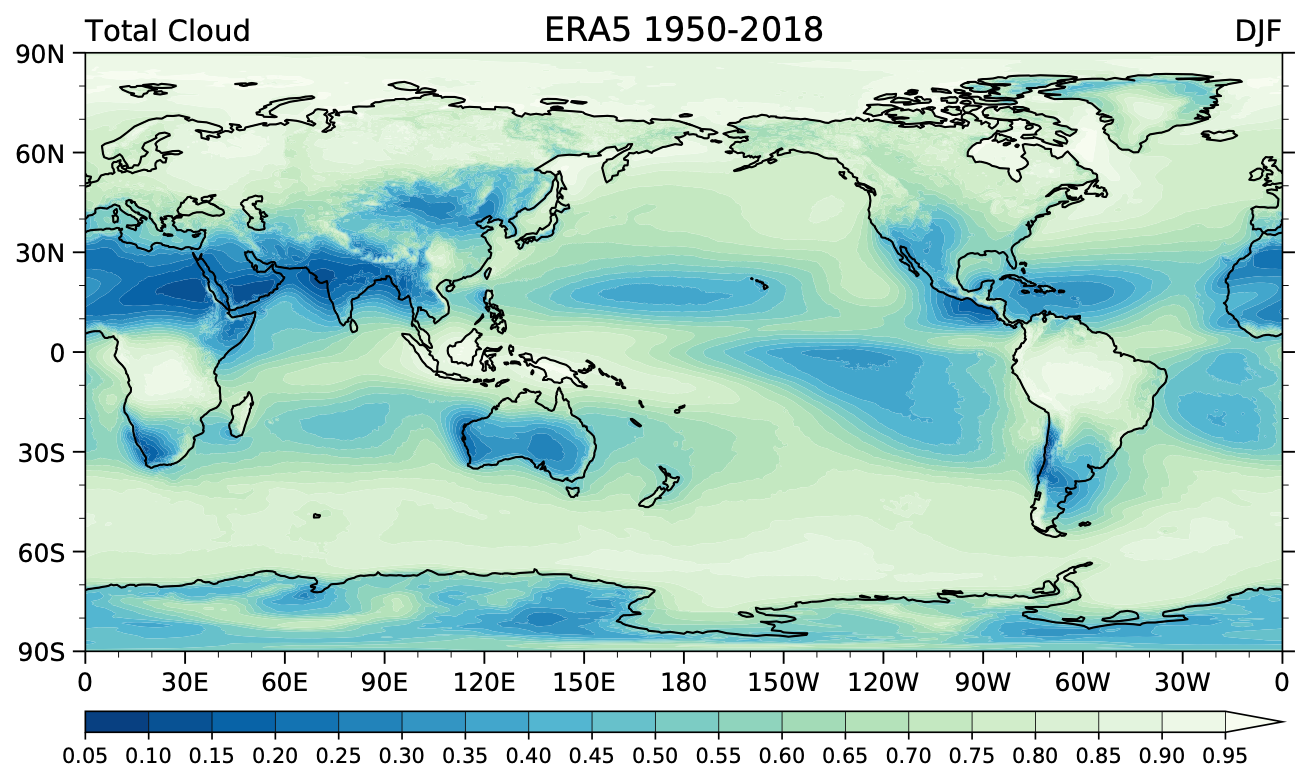
\includegraphics[width = .7 \textwidth]{figs/GD/CloudsDJF.png}
\caption{Total cloud cover for Winter (DJF)}
\end{figure}

\begin{figure}
\centering
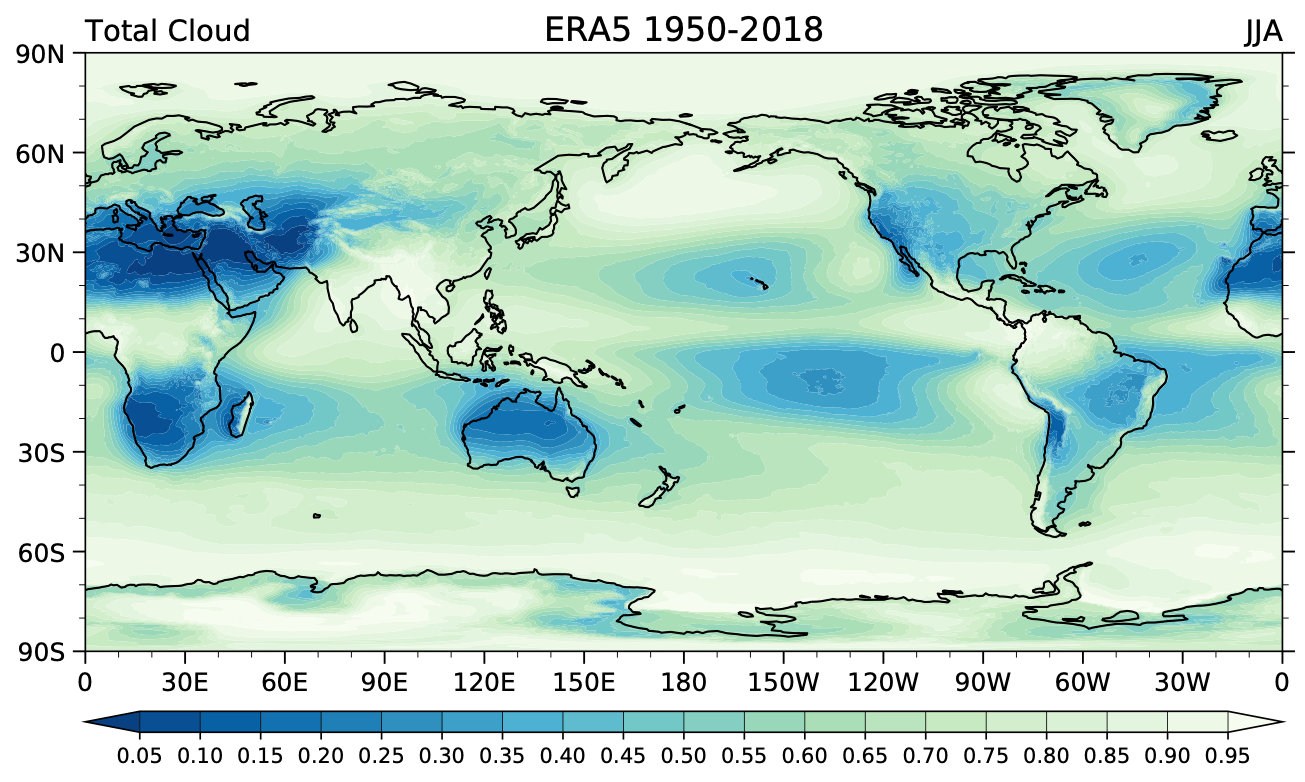
\includegraphics[width = .7 \textwidth]{figs/GD/CloudsJJA.png}
\caption{As in Fig. \texttt{fig:772} but for Summer (JJA)}
\label{fig:}
\end{figure}

It is interesting to look at the zonal profile of clouds. Fig.
(\texttt{fig:774}) shows clearly that concentration of clouds at the
equator and in the middle and high latitudes. The tropical desert zone
is also clearly visible. However, the cloud fraction can be misleading
with respect the actual amount of water present in the atmosphere. This
can be better investigated using the total column water content, as it
is shown in the picture, and then we can see that water is concentrated
in the equatorial zone and then a relatively small portion of water is
present in the atmosphere outside this zone.

\begin{figure}
\centering
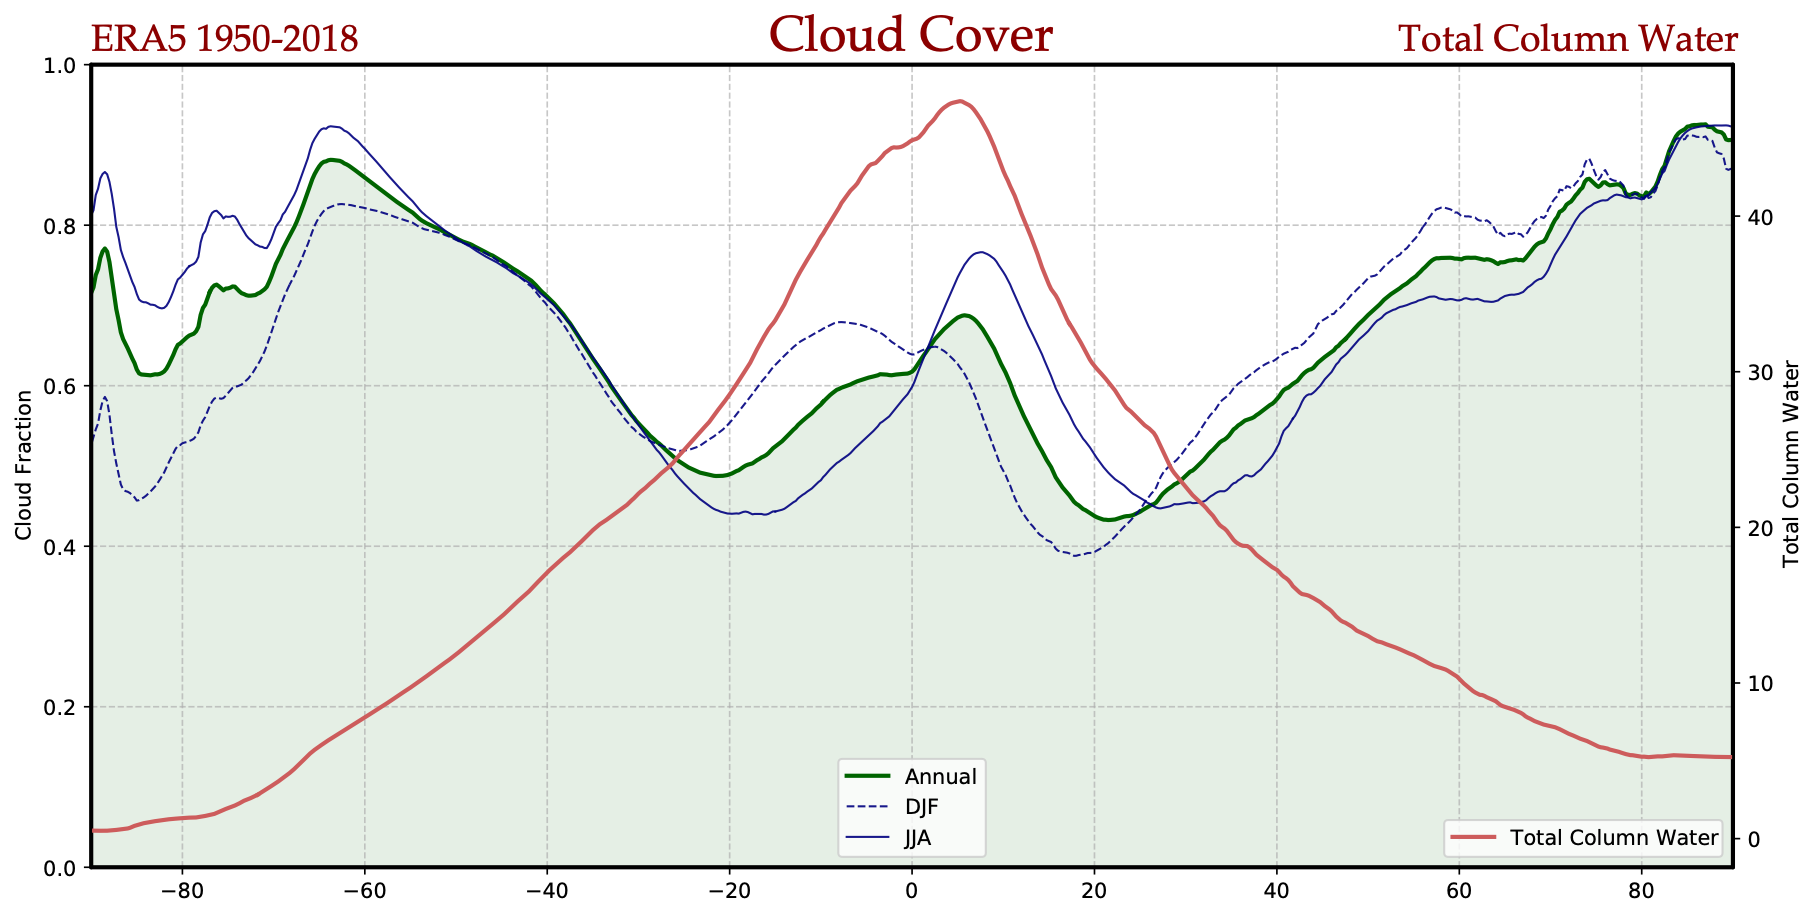
\includegraphics[width = .7 \textwidth]{figs/GD/CloudsProfile.png}
\caption{} \label{fig:}
\end{figure}
